\chapter{Análise dos Resultados} \label{ch:resultados}
\setlength{\headheight}{13.6pt}
%%%%%%%%%%%%%%%%%%%%%%%%%%%%%%%%%%%%%%%%%%%%%%%%%%%%%
Conforme referido no Capítulo \ref{ch:intro}, o presente capítulo é dedicado à apresentação e discussão dos resultados obtidos através das simulações e experiências conduzidas ao longo do desenvolvimento do projeto da ferramenta porta-peças.
\par
Para facilitar a discussão, os resultados serão apresentados apenas para uma série de rodas de coroa, nomeadamente a série DB45. Esta escolha fundamentou-se na disponibilidade dos resultados, dado que este foi o primeiro conjunto de testes a ser realizado e os seus resultados já estavam disponíveis para análise aquando da elaboração deste documento. Pouco antes da finalização deste documento, obtiveram-se também os resultados das rodas de coroa da série JT4. No entanto, os resultados relativos à série DB35 apenas estarão disponíveis após a data de entrega deste documento.

\par
Para os resultados das simulações, foi necessário calcular as temperaturas de austenitização A\textsubscript{C1} e A\textsubscript{C3} do material, com base nas Equações \ref{eq:A_C1} e \ref{eq:A_C3}, respetivamente. A Tabela \ref{tab:temp_sim} apresenta estes valores, assim como outros dados relevantes para a análise dos resultados das simulações que serão discutidos na secção seguinte, a Secção \ref{sec:resultados_simulacoes}.
%%%%%%%%%%%%%%%%%%%%%%%%%%%%%%%%%%%%%%%%%%%%%%%%%%%%%%%%%%%%%%%%%%%%%%%%%%%%%
\begin{table}[htb]
    \centering
    \caption[Valores de temperatura importantes para a análise de resultados]%
    {Valores de temperaturas críticas, para o Aço 27MC5, antes e após a carbonitruração, respetivamente, importantes para a análise de resultados.}
    \label{tab:temp_sim}
    \begin{tabular}{lrr} 
    \toprule
    \textbf{Ponto Crítico}                  & \multicolumn{1}{c}{\textbf{Temperatura\textsubscript{Base}}} & \multicolumn{1}{c}{\textbf{Temperatura\textsubscript{(Carb.)}}}  \\ 
    \hline\hline
    Início de Austenitização \textbf{(A\textsubscript{C1})} & 707 °C                                            & 707 °C                                               \\
    Final de Austenitização \textbf{(A\textsubscript{C3})}  & 788 °C                                            & 715 °C                                               \\
    Início de Martensite \textbf{(M\textsubscript{S})}      & 370 °C                                            & 188 °C                                               \\
    Final de Martensite \textbf{(M\textsubscript{F})}       & 175 °C                                            & -30 °C                                               \\
    \hline
    Início de Têmpera \textbf{(T\textsubscript{0})}         & \multicolumn{2}{c}{870 °C}                                                                                \\
    Final de Têmpera \textbf{(T\textsubscript{F})}          & \multicolumn{2}{c}{170 °C}                                                                                \\
    \bottomrule
    \end{tabular}
    \end{table}
%%%%%%%%%%%%%%%%%%%%%%%%%%%%%%%%%%%%%%%%%%%%%%%%%%%%%%%%%%%%%%%%%%%%%%%%%%%%%
\newpage
\section{Resultados das Simulações} \label{sec:resultados_simulacoes}
Foram apresentados alguns resultados das simulações no Capítulo \ref{ch:materiais} para assegurar uma sequência fluída do documento. Contudo, há outros resultados que exigem análise para se compreender a informação que se pode extrair das simulações numéricas.
\par
Tal como referido no capítulo anterior, executou-se uma simulação CFD para todos os protótipos desenvolvidos. Além do perfil das velocidades do fluido de têmpera, é possível extrair outros parâmetros por meio da simulação CFD. Por exemplo, pode-se obter os coeficientes de transferência de calor por convecção na interface entre os elementos finitos das rodas de coroa e os elementos finitos do fluido de têmpera. Estes valores podem ser introduzidos numa simulação transiente puramente térmica (ver Figura \ref{fig:simulacao_termica}), possibilitando a obtenção das velocidades de arrefecimento em vários pontos. Mais especificamente, consegue-se obter os valores da velocidade de arrefecimento num ponto dos dentes e num ponto do diâmetro interior.
%%%%%%%%%%%%%%%%%%%%%%%%%%%%%%%%%%%%%%%%%%%%%%%%%%
\begin{figure}[htb]
    \centering
    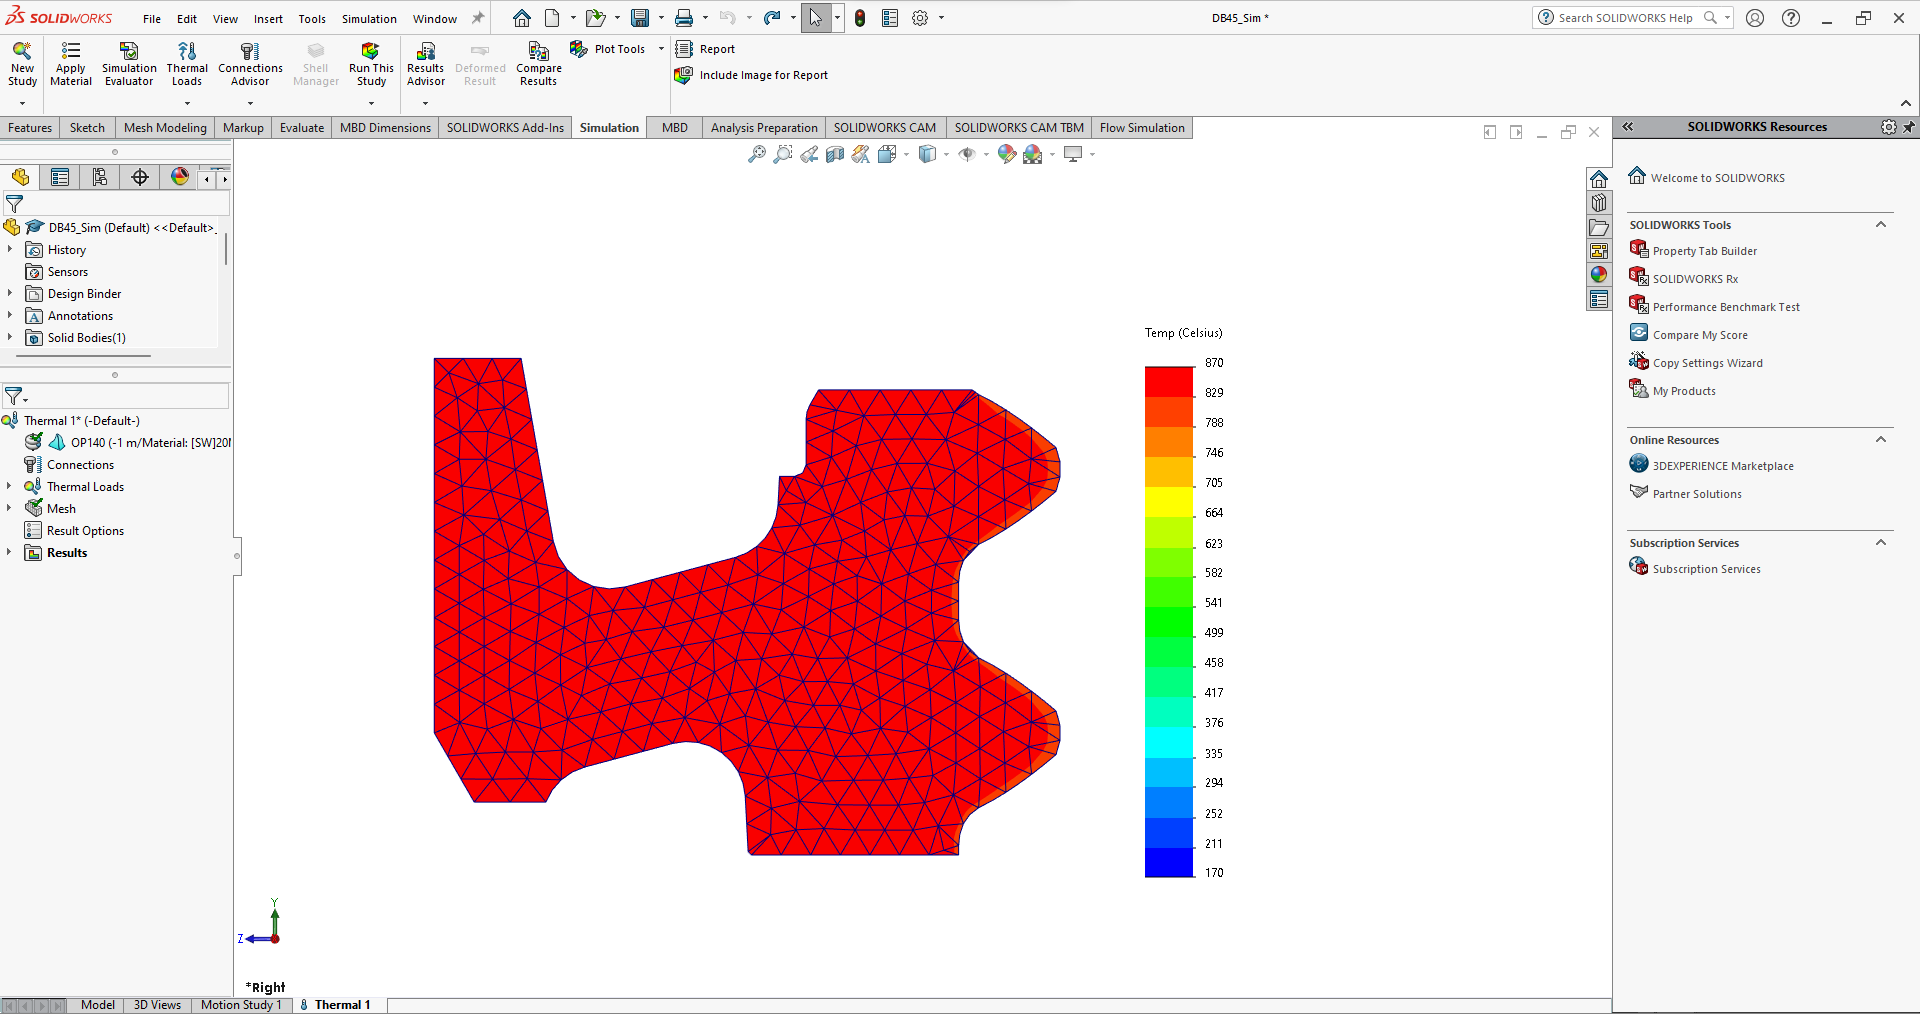
\includegraphics[width = 0.6\textwidth]{Figures/Cap4/Solidworks_thermal.png}
    \caption[Simulação puramente térmica Solidworks]%
    {Add-in do Solidworks simulation thermal para uma simulação puramente térmica.}
    \label{fig:simulacao_termica}
\end{figure}
%%%%%%%%%%%%%%%%%%%%%%%%%%%%%%%%%%%%%%%%%%%%%%%%%%%%%%%%%%%%%%%%%%%%%%%%%%%%%
\par
Após a execução da simulação, obtém-se dados temporais em seis locais distintos, três associados ao dentado e três ao diâmetro interno. O primeiro conjunto de dados corresponde ao momento em que os elementos alcançam a temperatura de austenitização A3, o segundo, ao momento em que atingem a temperatura de austenitização A1 e, finalmente, o terceiro corresponde ao instante em que os elementos atingem a temperatura de 170 \textdegree C. As Figuras \ref{fig:Dentado} ilustram os pontos de temperatura associados ao dentado, enquanto as Figuras \ref{fig:Diametro} apresentam os pontos de temperatura relacionados ao diâmetro interno das rodas de coroa.
\par
De forma a facilitar a visualização e otimizar o processamento, optou-se por focar exclusivamente na roda de coroa número 6, ou seja, a roda central da coluna. As simulações foram realizadas em um modelo de corte por simetria, utilizando elementos bidimensionais, com o intuito de reduzir a quantidade de elementos necessários em cada simulação. A tabela \ref{tab:pontos_sim} mostra os valores dos pontos e o tempo correspondente a cada um deles, extraídos diretamente das imagens. A partir destes dados, torna-se possível determinar a taxa de arrefecimento nos pontos especificados e, consequentemente, estimar a microestrutura final tanto no dentado como no diâmetro interno. Adicionalmente, é possível prever a dureza final em ambos os pontos, considerando a microestrutura, a taxa de arrefecimento e a composição química do material.
\newpage
%%%%%%%%%%%%%%%%%%%%%%%%%%%%%%%%%%%%%%%%%%%%%%%%%%%%%%%%%%%%%%%%%%%%%%%%%%%%%
\begin{figure}[htb]
    \centering
    \begin{subfigure}{.33\textwidth}\
        \centering
        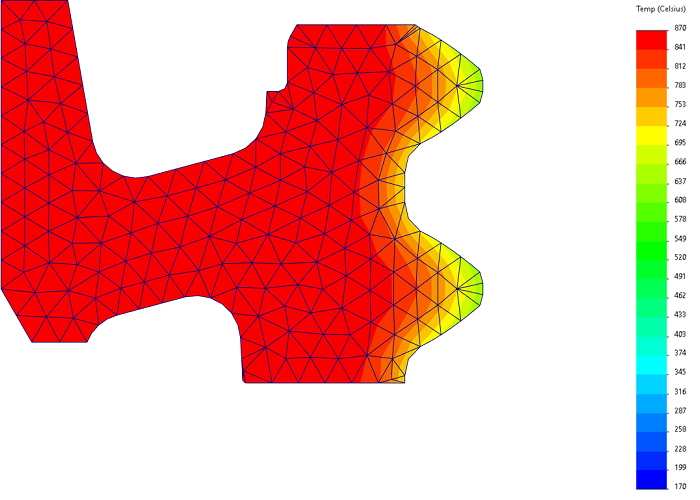
\includegraphics[width = 0.8\textwidth]{Figures/Cap4/AC3_Dentado.png}
        \caption[]%
        {}
        \label{fig:A3_Dent}
    \end{subfigure}%
    \begin{subfigure}{.33\textwidth}
        \centering
        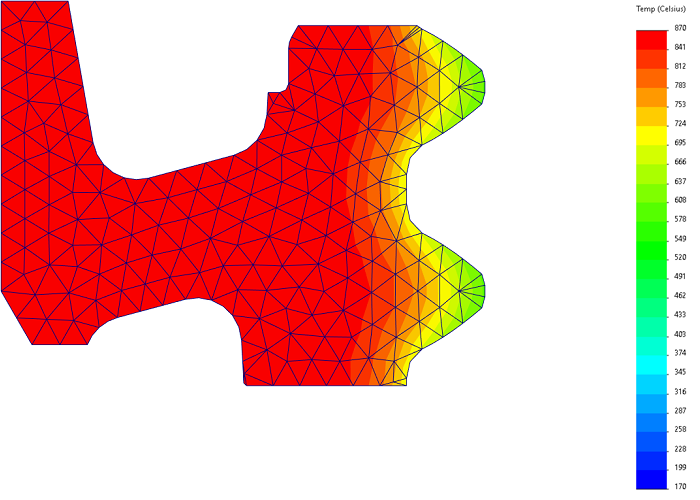
\includegraphics[width = 0.8\textwidth]{Figures/Cap4/AC1_Dentado.png}
        \caption{}
        \label{fig:A1_Dent}
    \end{subfigure}
    \begin{subfigure}{.33\textwidth}
        \centering
        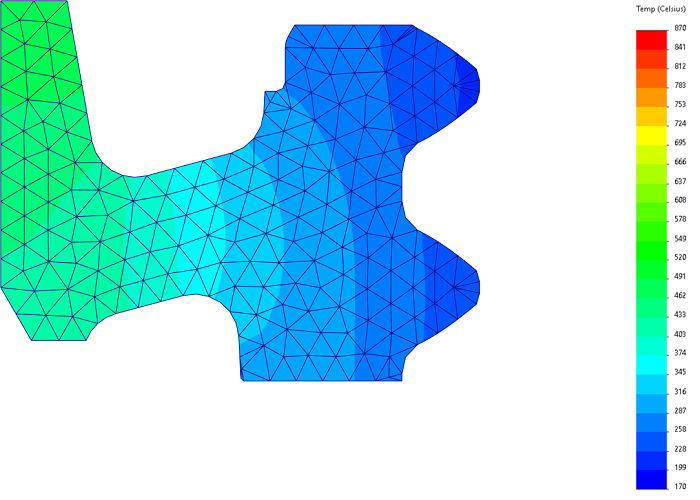
\includegraphics[width = 0.8\textwidth]{Figures/Cap4/TF_Dentado.png}
        \caption{}
        \label{fig:Tf_Dent}
    \end{subfigure}
    \caption[Pontos críticos dos elementos finitos do dentado]%
    {Pontos críticos dos elementos finitos do dentado, para obtenção dos valores de tempo. À esquerda, temperatura A\textsubscript{C1}, que ocorre aos 0,45s, no centro, temperatura A\textsubscript{C3}, que ocorre aos 3,05 s, e à direita, temperatura T\textsubscript{F}, aos 52,00s.}
    \label{fig:Dentado}
\end{figure}
%%%%%%%%%%%%%%%%%%%%%%%%%%%%%%%%%%%%%%%%%%%%%%%%%%%%%%%%%%%%%%%%%%%%%%%%%%%%%
%%%%%%%%%%%%%%%%%%%%%%%%%%%%%%%%%%%%%%%%%%%%%%%%%%%%%%%%%%%%%%%%%%%%%%%%%%%%%
\begin{figure}[htb]
    \centering
    \begin{subfigure}{.33\textwidth}\
        \centering
        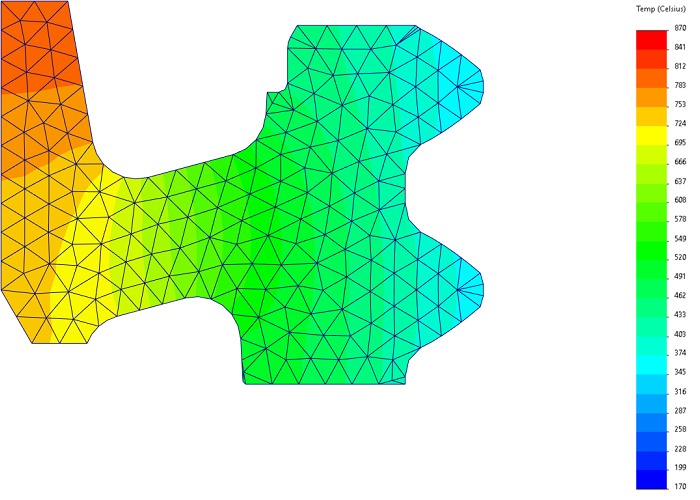
\includegraphics[width = 0.8\textwidth]{Figures/Cap4/AC3_Diametro.png}
        \caption[]%
        {}
        \label{fig:A3_Dint}
    \end{subfigure}%
    \begin{subfigure}{.33\textwidth}
        \centering
        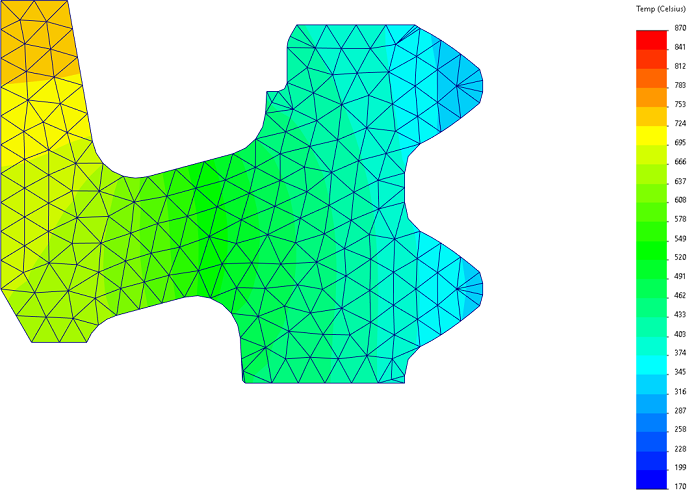
\includegraphics[width = 0.8\textwidth]{Figures/Cap4/AC1_Diametro.png}
        \caption{}
        \label{fig:A1_Dint}
    \end{subfigure}
    \begin{subfigure}{.33\textwidth}
        \centering
        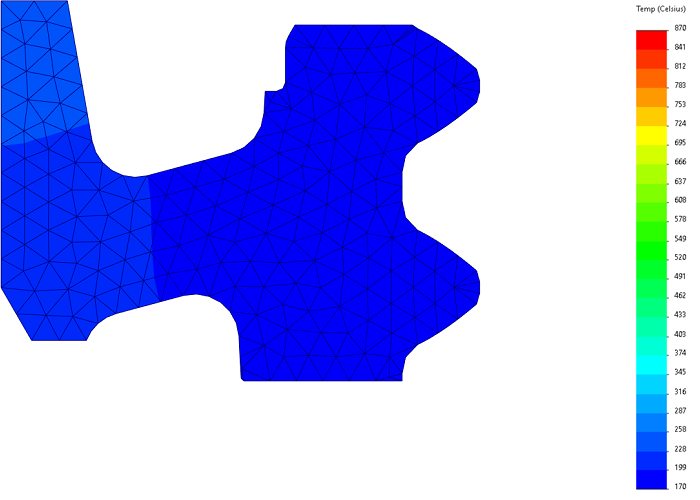
\includegraphics[width = 0.8\textwidth]{Figures/Cap4/TF_Diametro.png}
        \caption{}
        \label{fig:Tf_Dint}
    \end{subfigure}
    \caption[Pontos críticos dos elementos finitos do diâmetro interno]%
    {Pontos críticos dos elementos finitos do diâmetro interno, para obtenção dos valores de tempo. À esquerda, temperatura A\textsubscript{C1}, que ocorre aos 27,65s, no centro, temperatura A\textsubscript{C3}, que ocorre aos 47,15 s, e à direita, temperatura T\textsubscript{F}, aos 170,00s.}
    \label{fig:Diametro}
\end{figure}
%%%%%%%%%%%%%%%%%%%%%%%%%%%%%%%%%%%%%%%%%%%%%%%%%%%%%%%%%%%%%%%%%%%%%%%%%%%%%
\par
Nota-se que se utilizou uma taxa de carbono de 0,7\% para o sector dentado e de 0,24\% para o diâmetro interno. Contudo, convém enfatizar que a garantia de ausência de enriquecimento de carbono no diâmetro interno é algo que não se pode assegurar completamente. Dada a impossibilidade de antecipar o valor final da percentagem de carbono no diâmetro interno, optou-se pela aplicação do valor inerente ao material de base. Considerando os valores alcançados, torna-se viável estimar uma velocidade média de arrefecimento na ordem dos 35,0°C/s para o sector dentado e uma velocidade média de arrefecimento de 4,7°C/s para o diâmetro interno.
\par
Em relação ao sector dentado, prevê-se níveis de dureza na casa dos 860HV para uma microestrutura maioritariamente martensítica e 290HV para uma microestrutura maioritariamente ferrítica e perlítica. Para o diâmetro interno, e assumindo a ausência de enriquecimento, prevê-se que uma estrutura maioritariamente martensítica possua níveis de dureza na ordem dos 500HV, enquanto uma estrutura maioritariamente ferrítica e perlítica deverá apresentar uma dureza aproximada de 190HV.
%%%%%%%%%%%%%%%%%%%%%%%%%%%%%%%%%%%%%%%%%%%%%%%%%%%%%%%%%%%%%%%%%%%%%%%%%%%%%
\begin{table}[htb]
    \centering
    \refstepcounter{table}
    \caption[Valores temporais para cada temperatura crítica]{Valores temporais para cada temperatura crítica no dentado e no diâmetro interno.}
    \label{tab:pontos_sim}
    \begin{tabular}{lr} 
    \toprule
    \multicolumn{1}{c}{\textbf{Ponto Crítico}}            & \multicolumn{1}{c}{\textbf{Tempo (s)}}                         \\ 
    \hline\hline
    Início de Têmpera (T\textsubscript{0})                                & 0,00 s                                         \\ 
    \hline
    Final de Austenitização no dentado (A\textsubscript{C3\_t})           & 0,45 s                                         \\
    Início de Austenitização no dentado (A\textsubscript{C1\_t})          & 3,05 s                                         \\
    Final de Têmpera no dentado (T\textsubscript{F\_t})                   & 52,00 s                                        \\ 
    \hline\hline
    Final de Austenitização no dentado (A\textsubscript{C3\_t})           & 27,65 s                                        \\
    Início de Austenitização no diâmetro interno (A\textsubscript{C1\_d}) & 47,15 s                                        \\ 
    Final de Têmpera (T\textsubscript{F\_d})                              & 170,00 s                                       \\
    \bottomrule
    \end{tabular}
\end{table}
%%%%%%%%%%%%%%%%%%%%%%%%%%%%%%%%%%%%%%%%%%%%%%%%%%%%%%%%%%%%%%%%%%%%%%%%%%%%%
\par
Considerando as velocidades de arrefecimento em questão, prevê-se que o setor dentado seja predominantemente composto por martensite, enquanto o diâmetro interno seja composto por ferrite e perlite. Nesse contexto, espera-se que as durezas estejam em torno de 860HV para o dentado e 190HV para o diâmetro interno. É válido ressaltar, no entanto, que essas estimativas são para o material que não foi submetido ao processo de revenido, no caso do dentado, e não sofreu enriquecimento de carbono, no caso do diâmetro interno. Caso o material seja submetido ao processo de revenido, é esperada uma redução nos níveis de dureza. De forma análoga, caso ocorra enriquecimento de carbono no diâmetro interno, espera-se um aumento nos níveis de dureza.
%%%%%%%%%%%%%%%%%%%%%%%%%%%%%%%%%%%%%%%%%%%%%%%%%%%%%%%%%%%%%%%%%%%%%%%%%%%%%
\section{Resultados do ensaio inicial} \label{sec:resultados_ensaio_inicial}

Conforme mencionado no Capítulo \ref{ch:materiais}, os resultados do protótipo inicial, mais especificamente da coluna protegida pela tampa P, ficaram aquém do esperado. A hipótese levantada para explicar esses resultados é que os três pontos de soldadura utilizados para unir a falsa coroa à torre, e isolar o diâmetro interno das coroas nessa coluna, sofreram rotura provavelmente devido à expansão térmica. De qualquer forma, as Figuras \ref{fig:resultados_Tampa_P_inicial} e \ref{fig:resultados_Serie_inicial} ilustram a diferença entre ter o diâmetro interno tamponado, e livre para a passagem do fluido de têmpera. Além disso, conforme observado nas Figuras \ref{fig:resultados_Tampa_P_inicial_dent} e \ref{fig:resultados_Serie_inicial_dent}, também é possível notar que o tamponamento do diâmetro interno não causa alterações significativas na dureza do dentado, o que confirma as vantagens da existência de uma ferramenta que protege o diâmetro interno das rodas de coroa.
%%%%%%%%%%%%%%%%%%%%%%%%%%%%%%%%%%%%%%%%%%%%%%%%%%%%%%%%%%%%%%%%%%%%%%%%%%%%%
\begin{figure}[htb]
    \centering
    \begin{subfigure}{.4\textwidth}
        \centering
        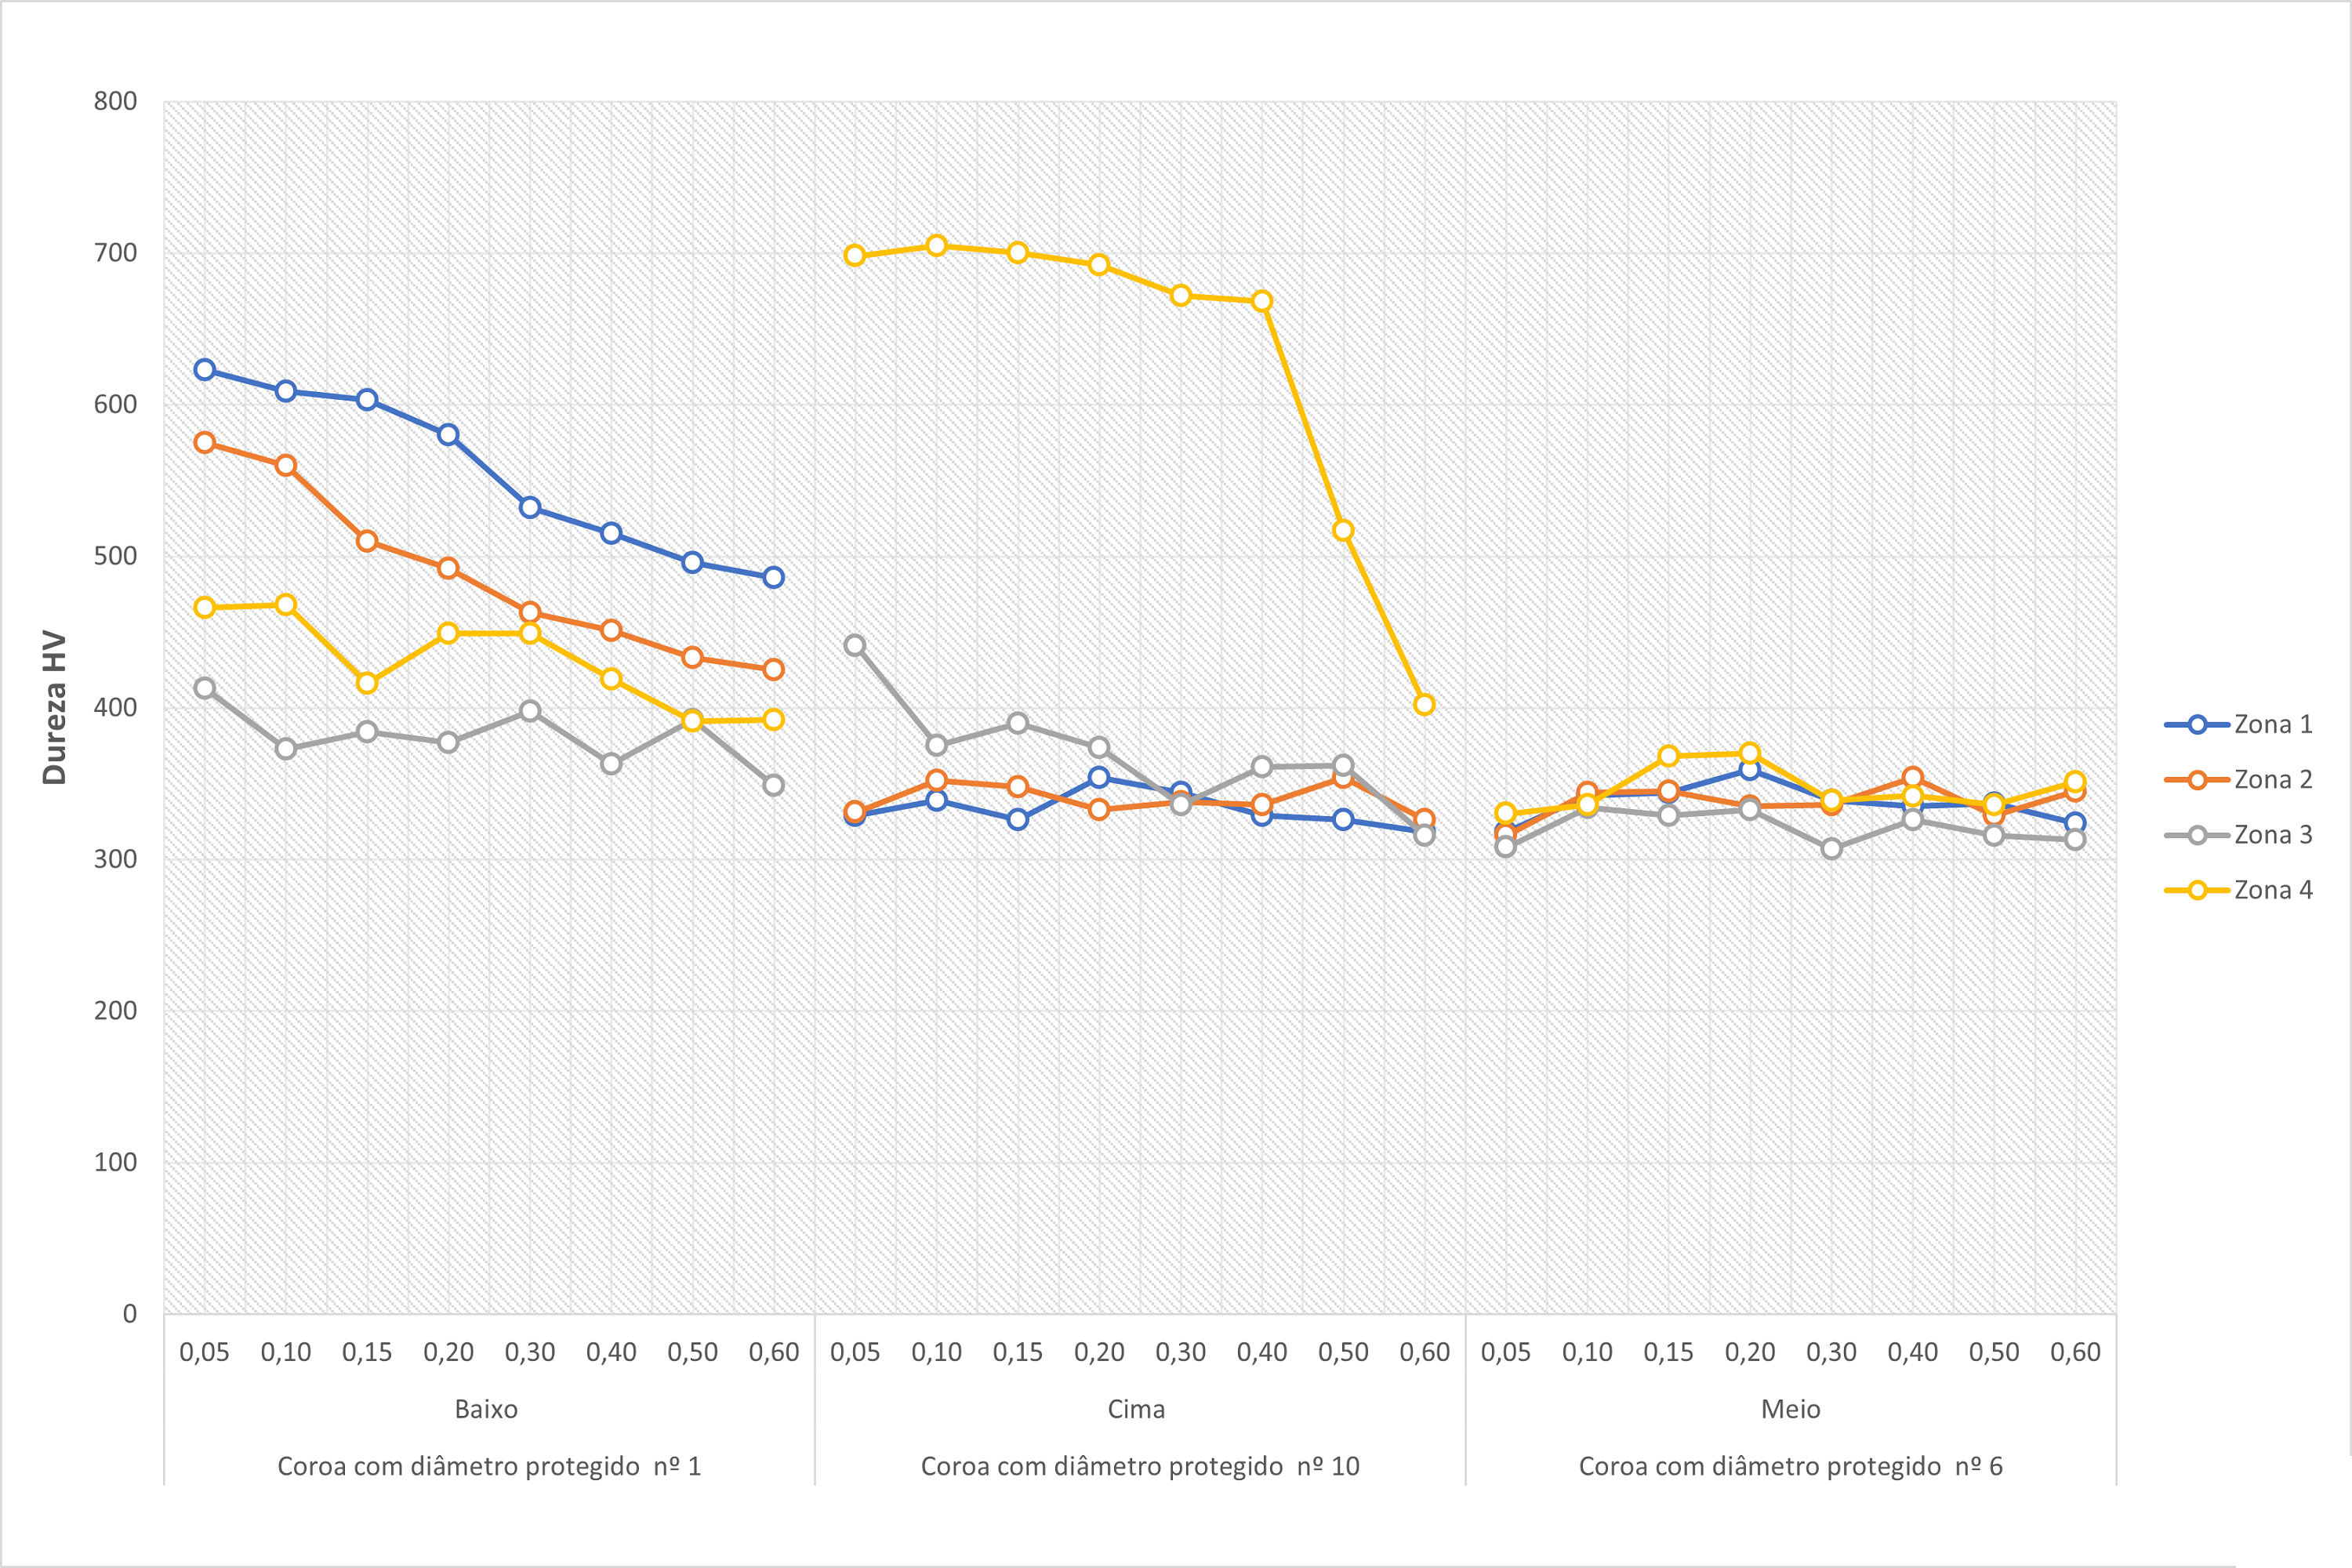
\includegraphics[width = 0.9\textwidth]{Figures/Cap4/Grafico_4_Zonas_P_inicial.png}
        \caption[]%
        {}
        \label{fig:resultados_Tampa_P_inicial}
    \end{subfigure}%
    \begin{subfigure}{.4\textwidth}
        \centering
        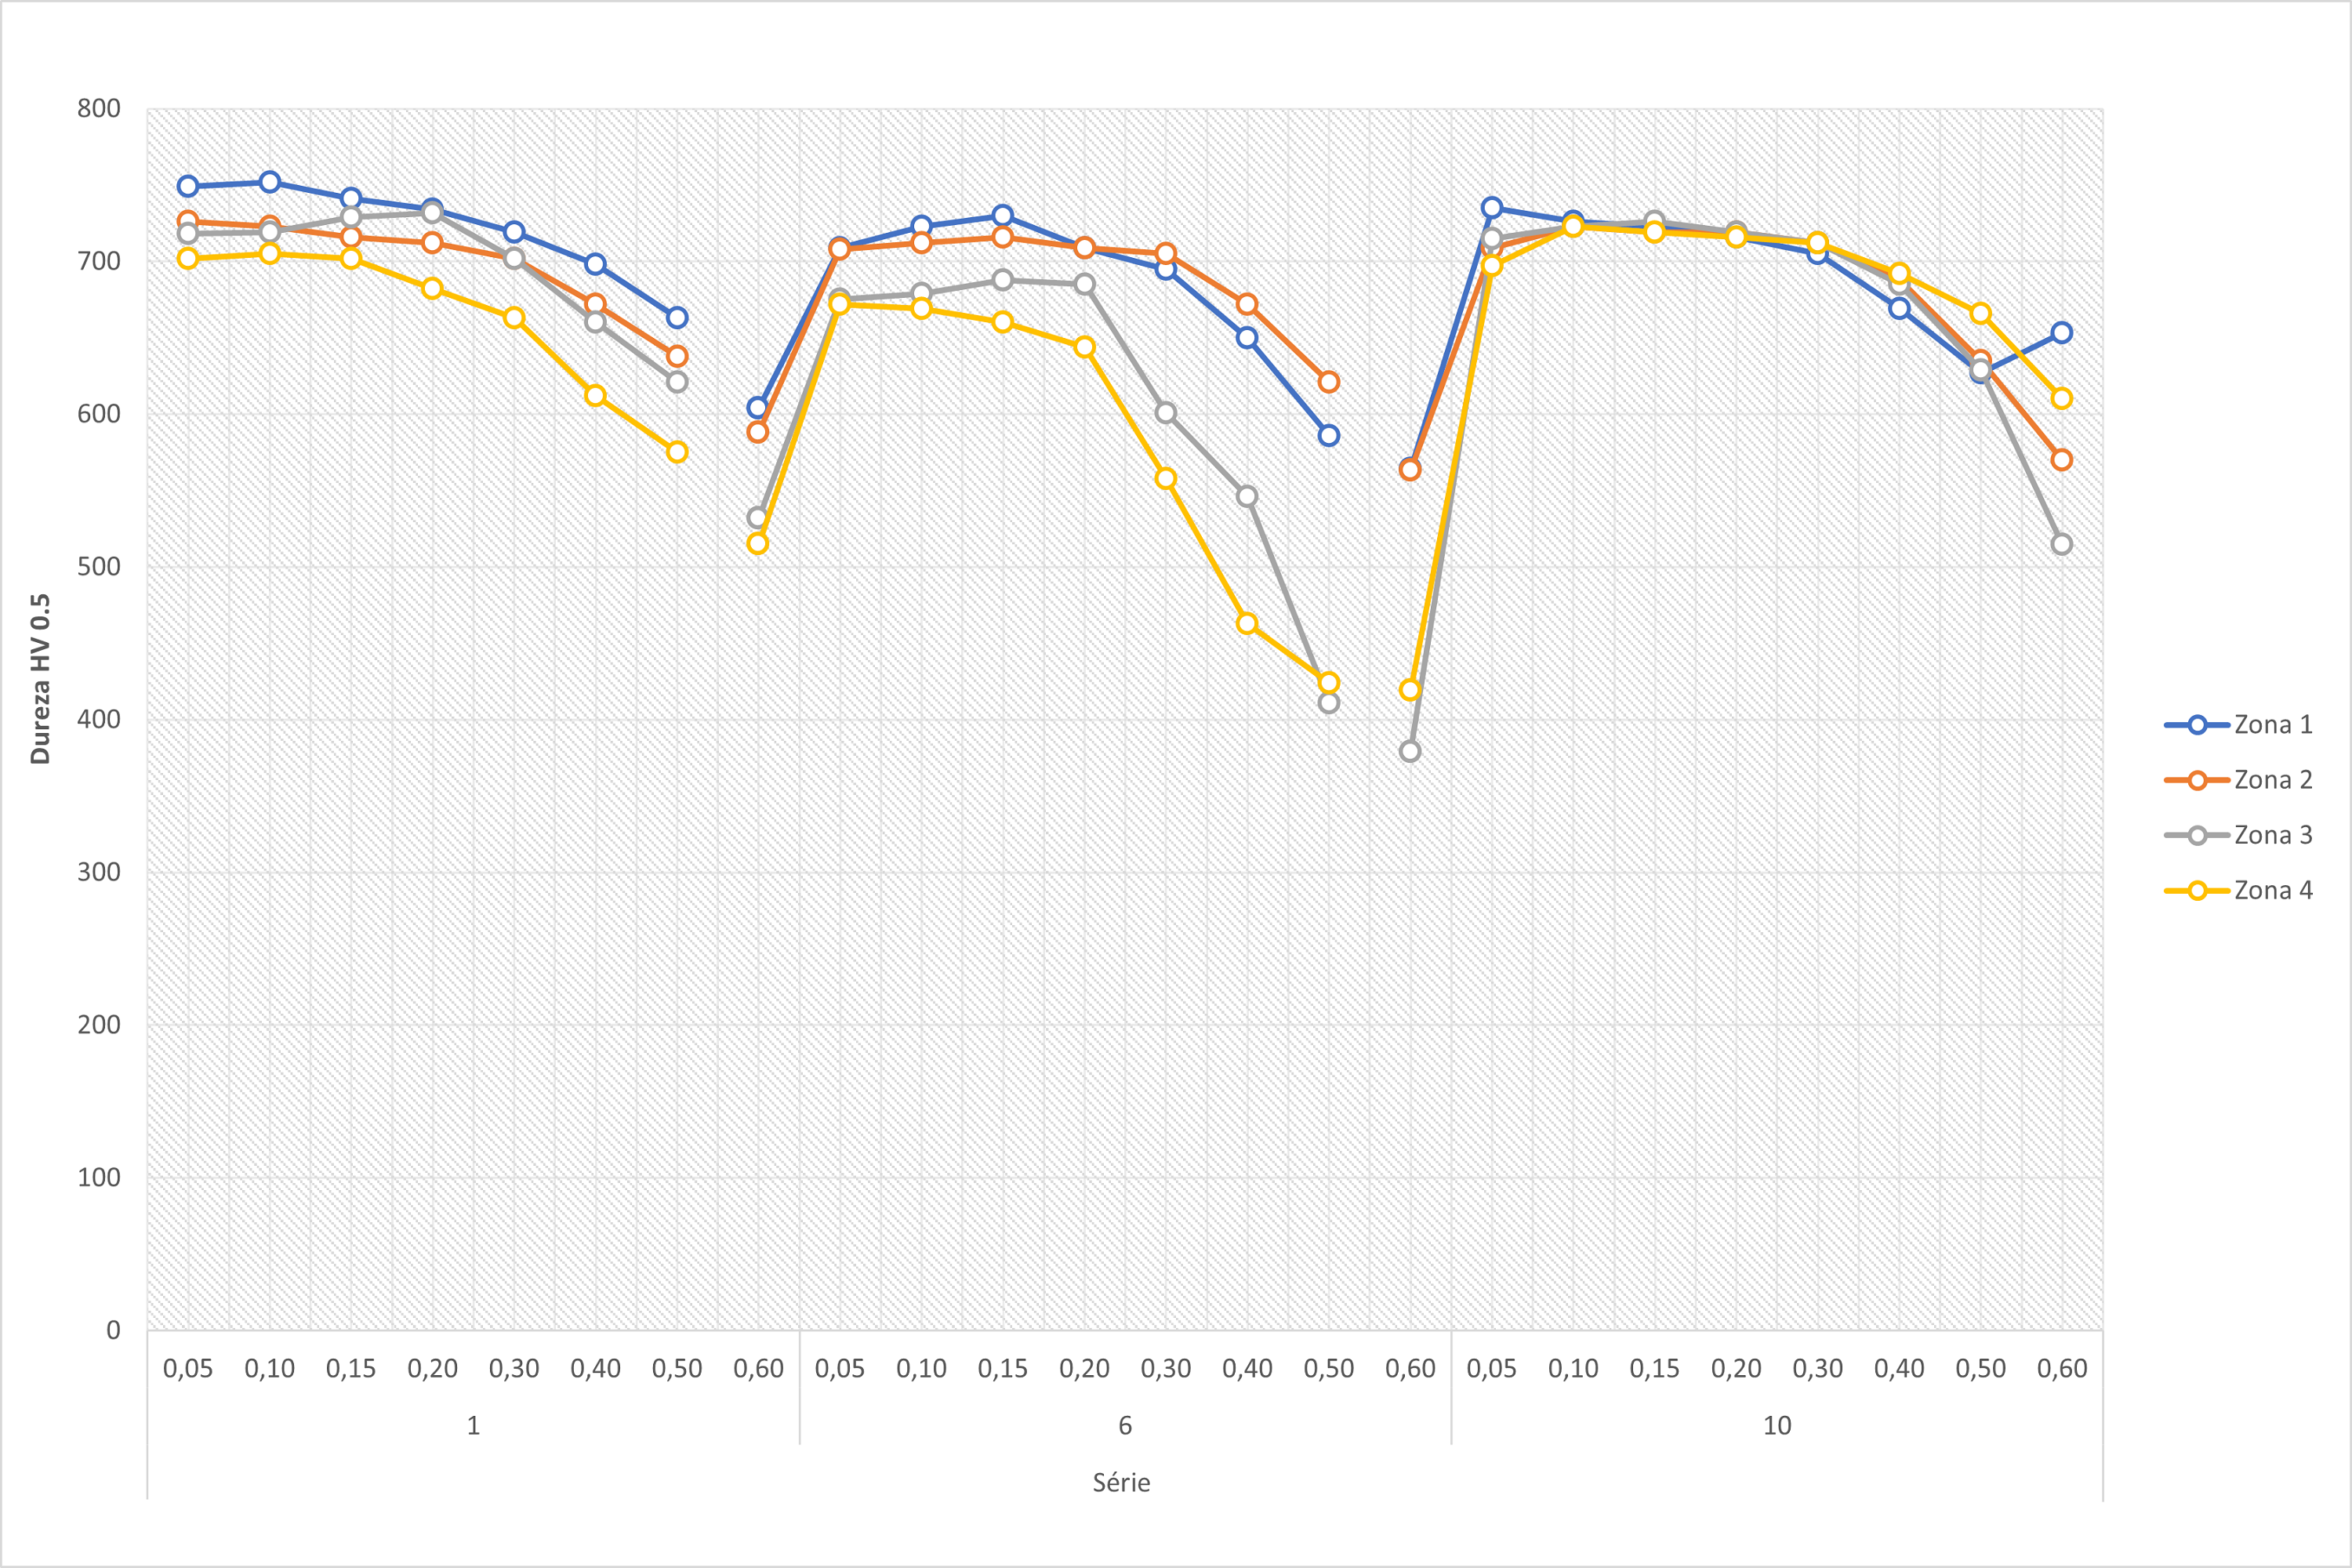
\includegraphics[width = 0.9\textwidth]{Figures/Cap4/Grafico_4_Zonas_S_inicial.png}
        \caption{}
        \label{fig:resultados_Serie_inicial}
    \end{subfigure}
    \begin{subfigure}{.4\textwidth}
        \centering
        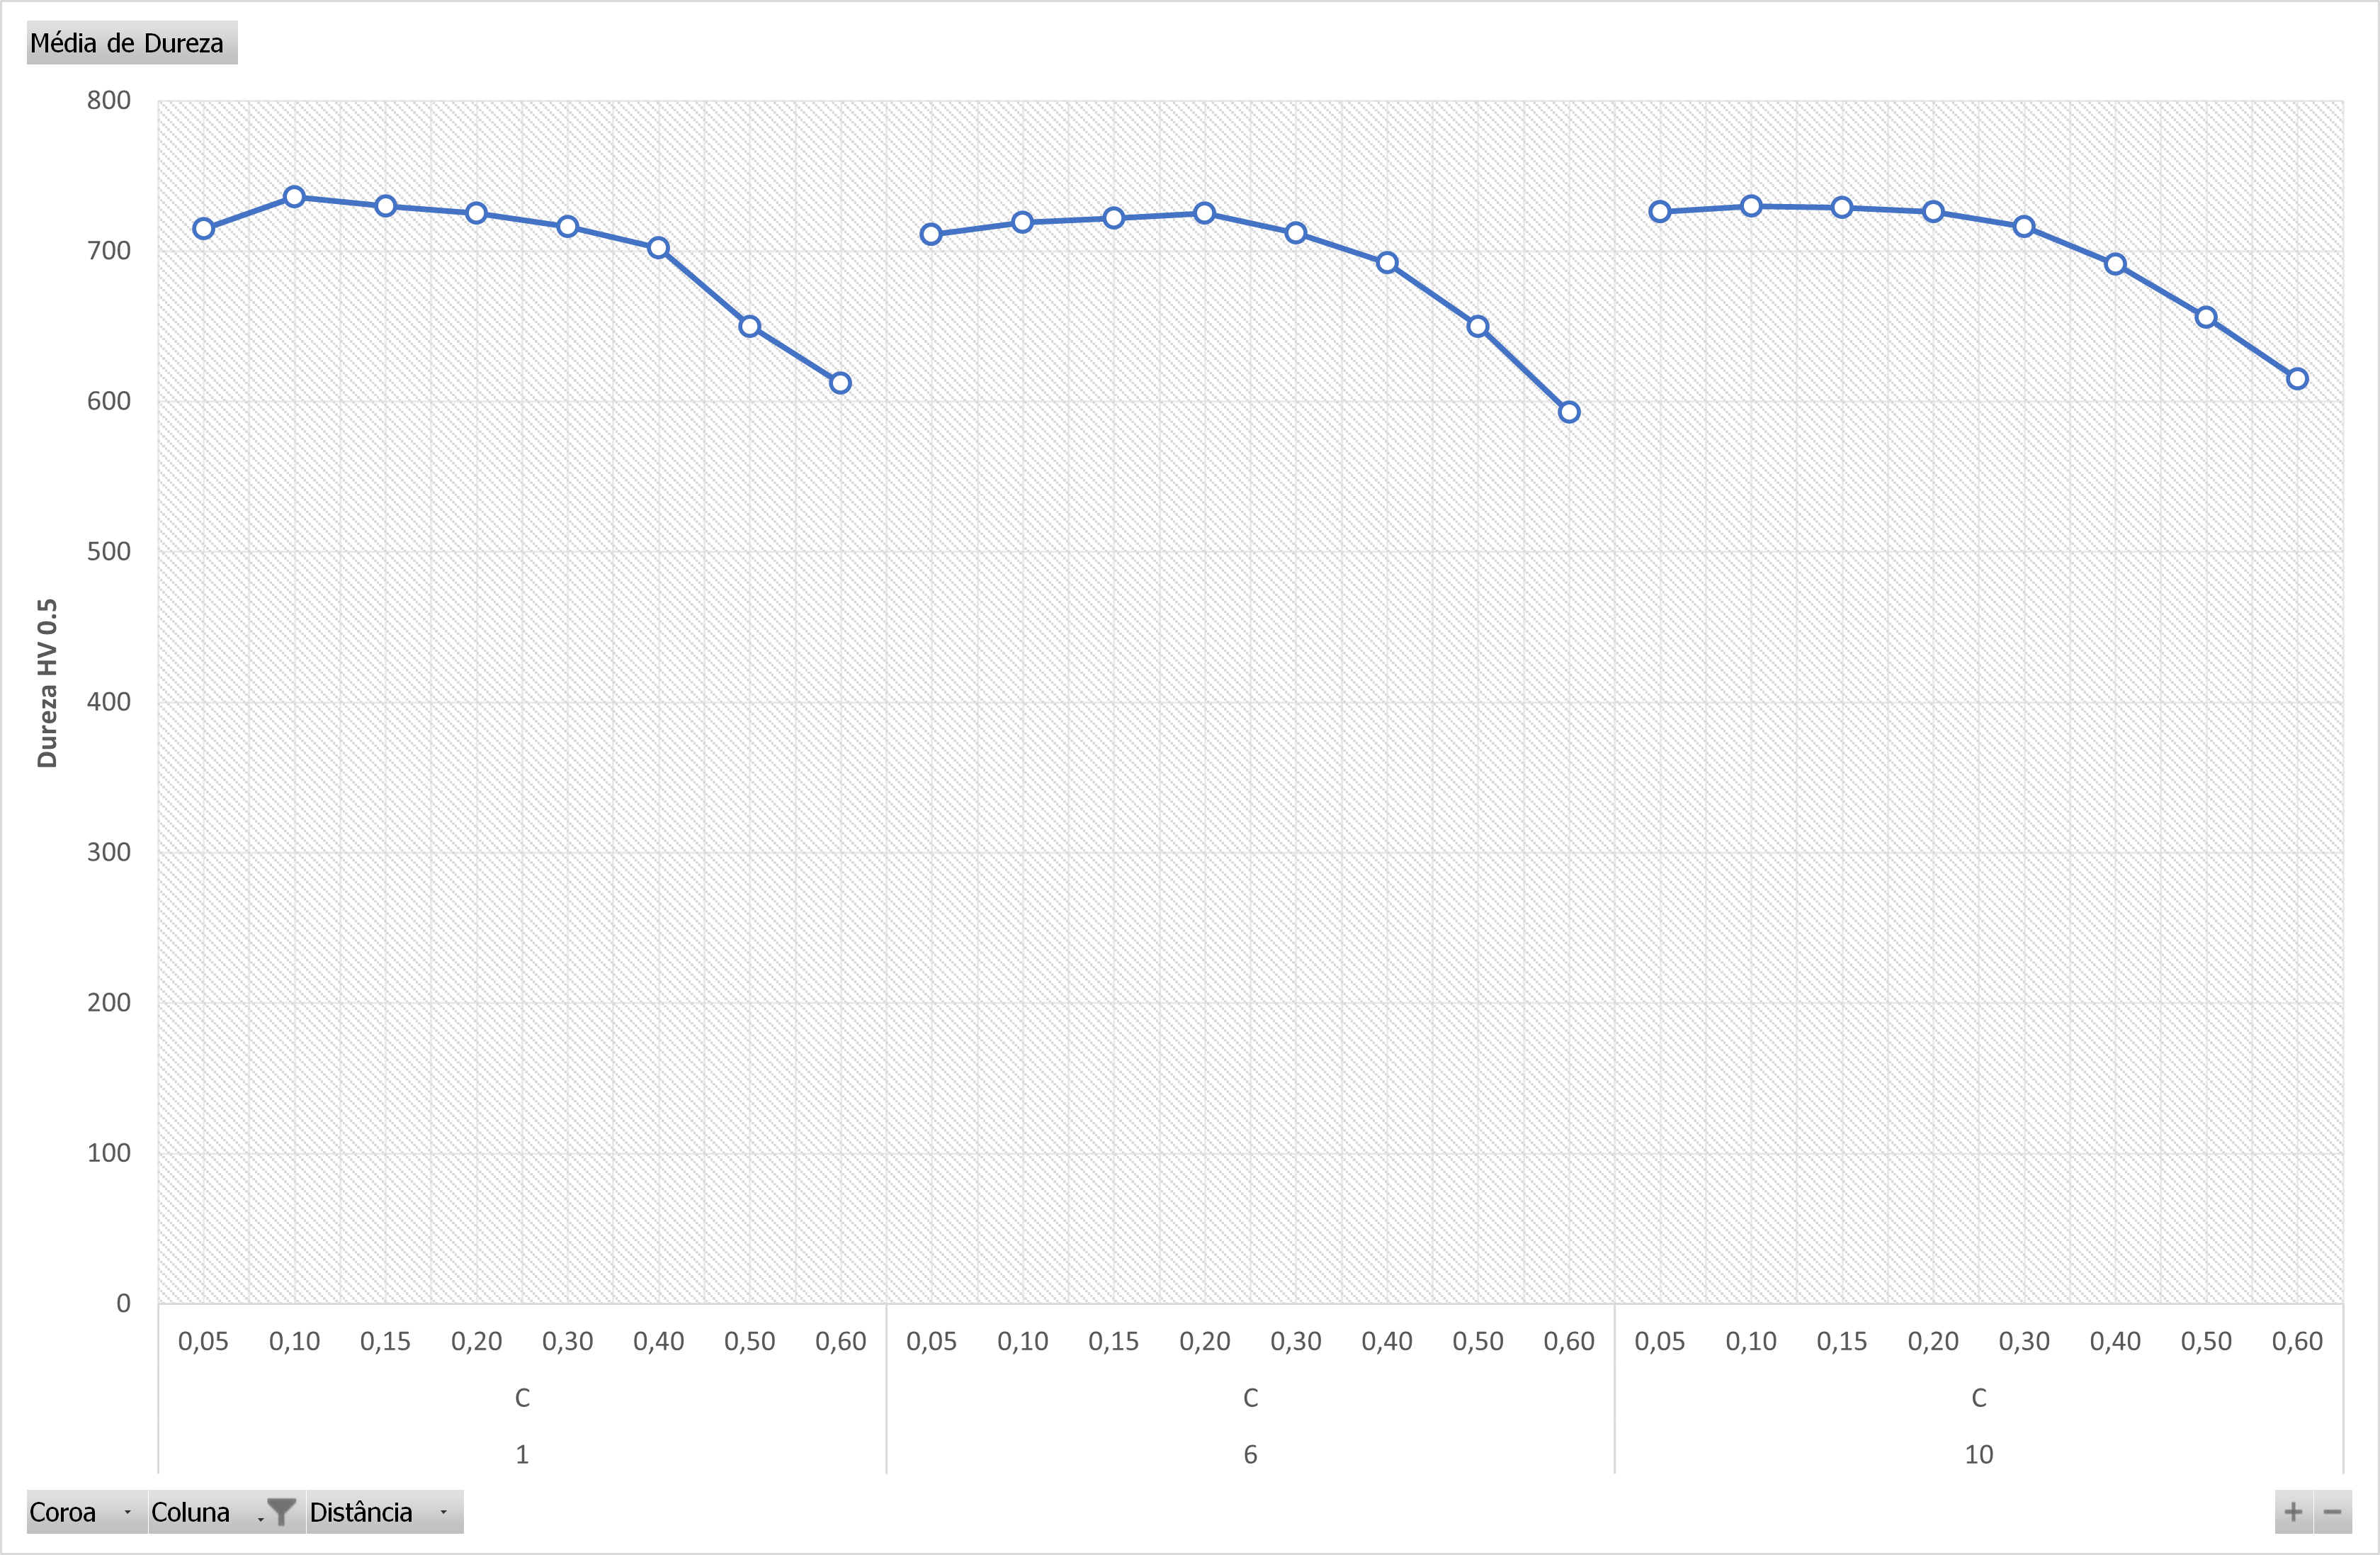
\includegraphics[width = 0.9\textwidth]{Figures/Cap4/Grafico_4_Zonas_P_inicial_dentado.png}
        \caption[]%
        {}
        \label{fig:resultados_Tampa_P_inicial_dent}
    \end{subfigure}%
    \begin{subfigure}{.4\textwidth}
        \centering
        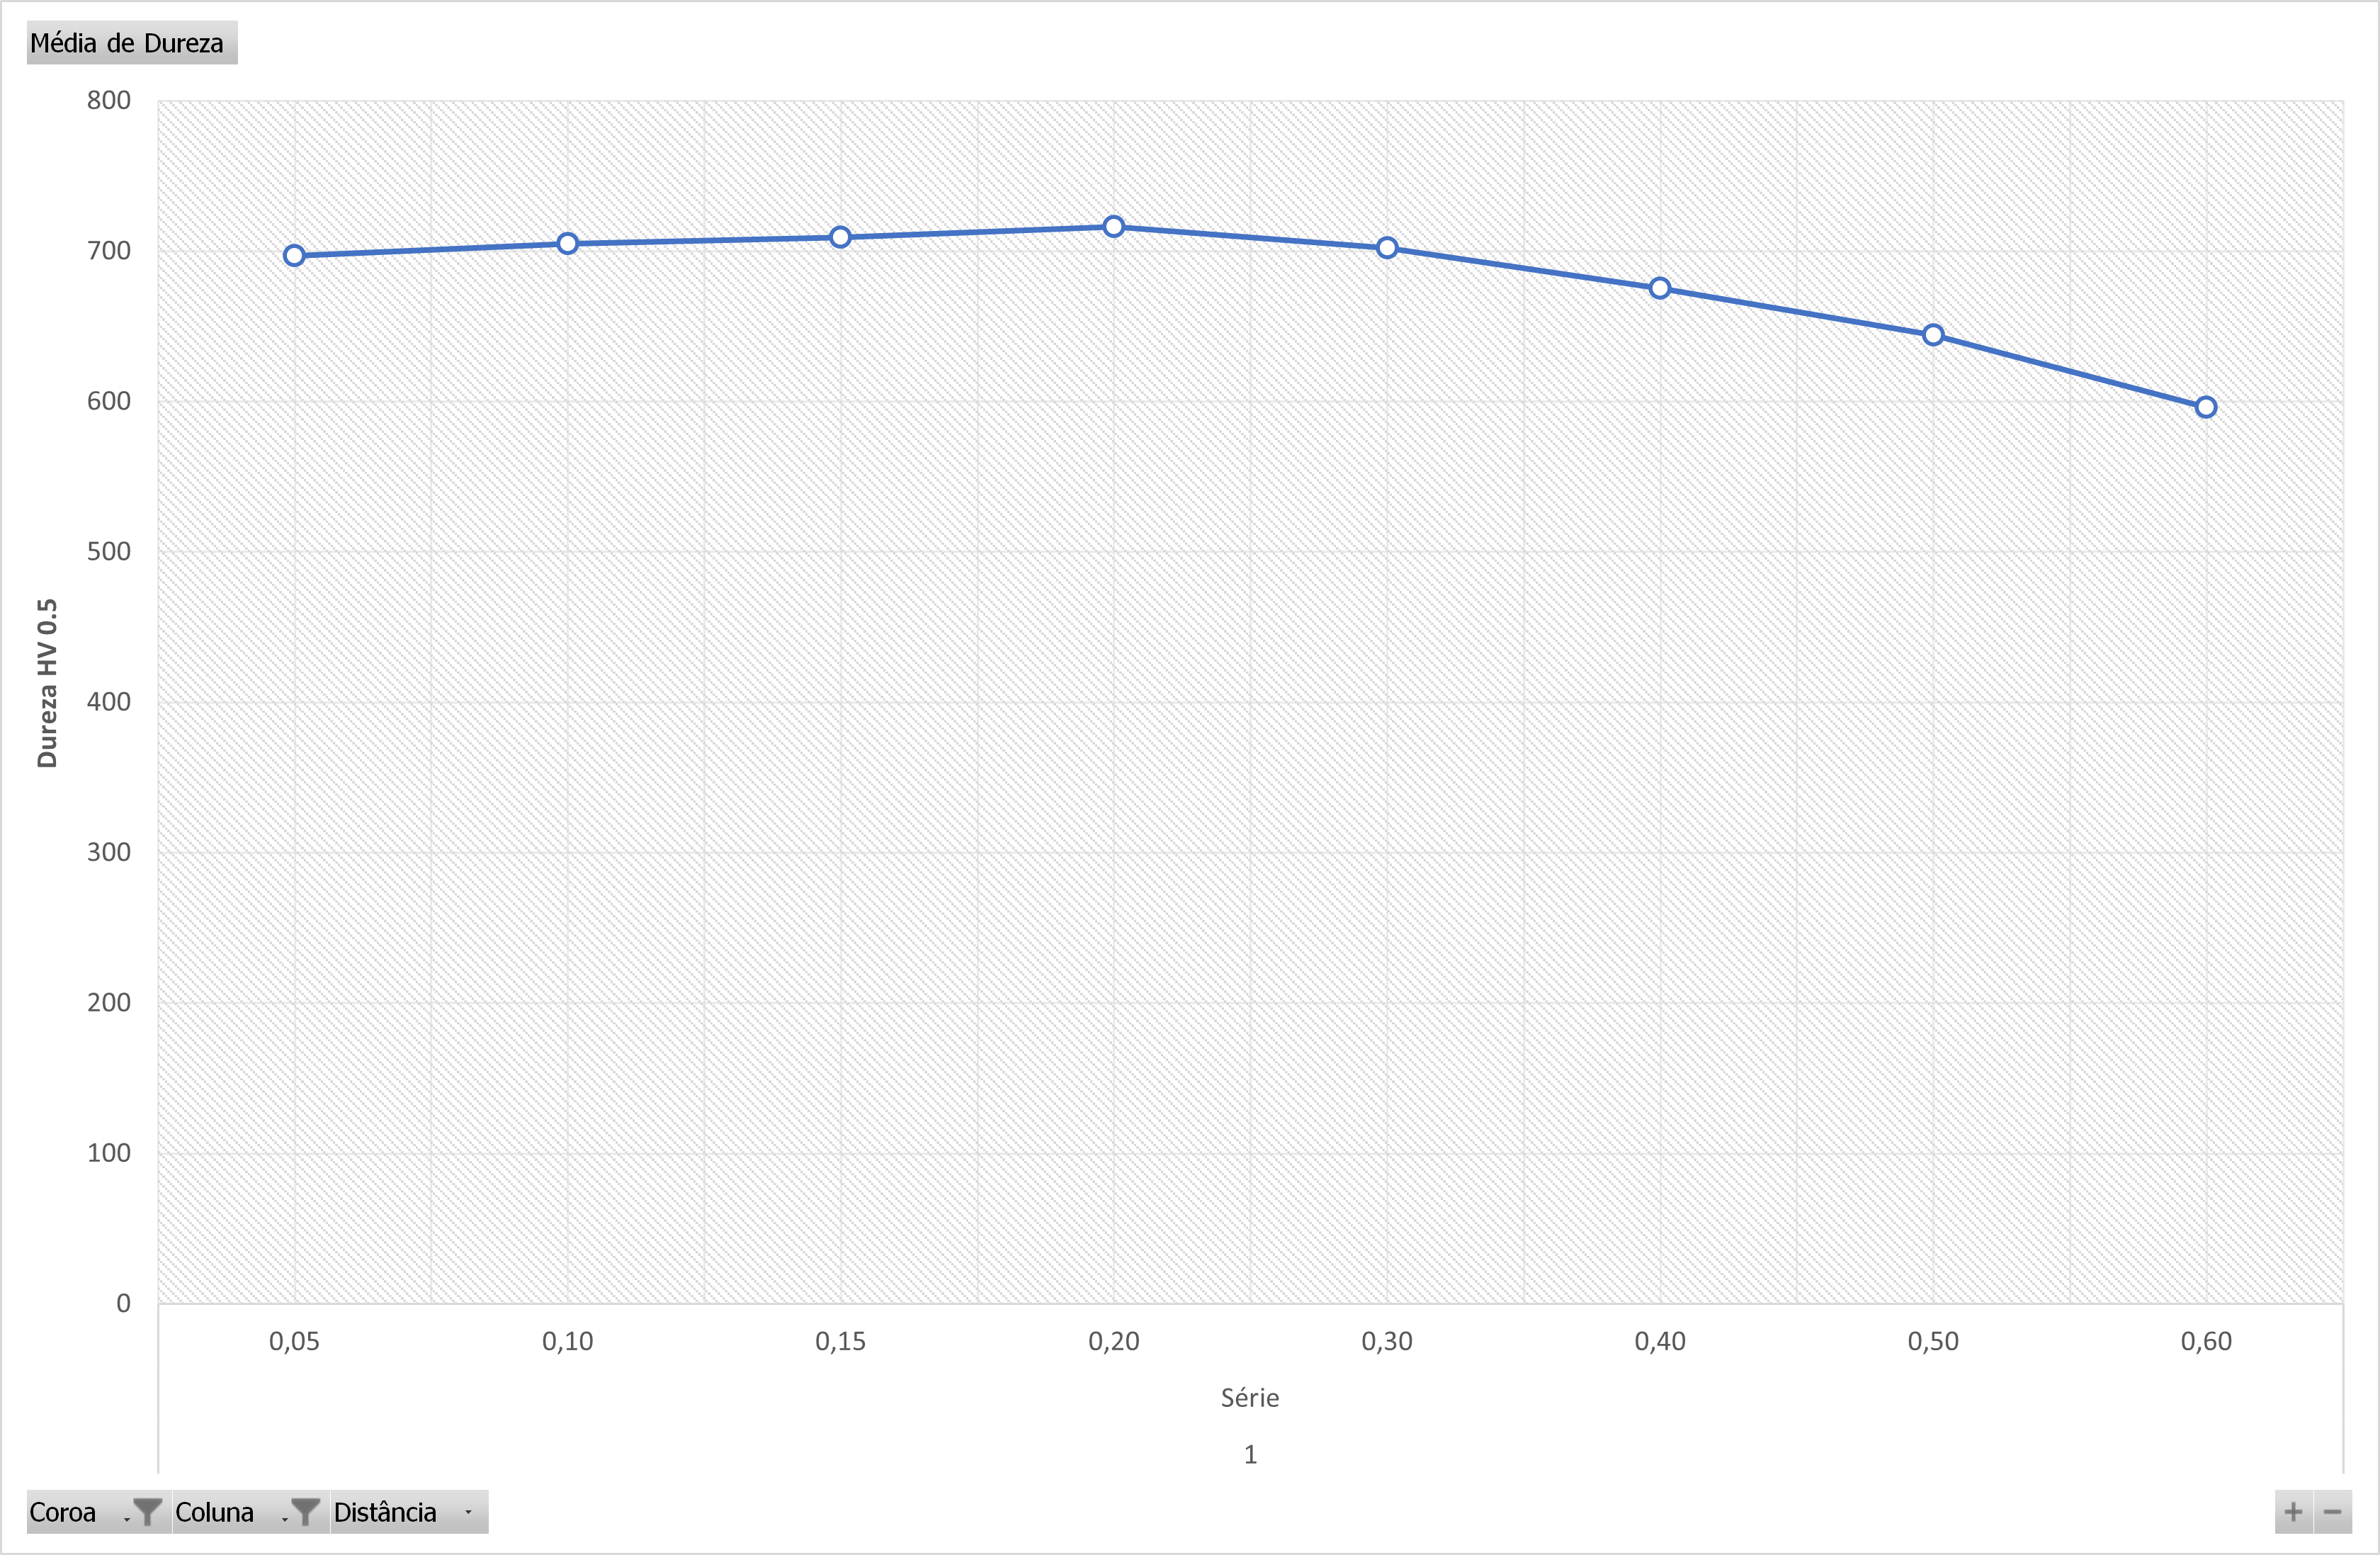
\includegraphics[width = 0.9\textwidth]{Figures/Cap4/Grafico_4_Zonas_S_inicial_dentado.png}
        \caption{}
        \label{fig:resultados_Serie_inicial_dent}
    \end{subfigure}
    \caption[Resultados do ensaio inicial e comparação com peças de série]%
    {Resultados das filiações de dureza obtidas no ensaio inicial, no diâmetro interno e no dentado, e comparação dos valores obtidos nos mesmos pontos nas peças de série.}
\end{figure}
%%%%%%%%%%%%%%%%%%%%%%%%%%%%%%%%%%%%%%%%%%%%%%%%%%%%%%%%%%%%%%%%%%%%%%%%%%%%%
\newpage
\par
É importante destacar que os valores de dureza encontrados no diâmetro interno estão consideravelmente acima dos valores teoricamente estimados, o que reforça a teoria de que há um enriquecimento de carbono nessa região das rodas de coroa protegidas. Outro fator relevante a ser mencionado é o ganho significativo de dureza na zona 4 da roda de coroa superior (número 1). Isso pode ser explicado pela geometria da tampa P, que faz contacto apenas nessa região, resultando em proteção parcial. Essa situação também explica a queda drástica na dureza a partir de 0,40 mm de profundidade. Por fim, observa-se o impacto da rotura da soldadura da falsa coroa na torre da ferramenta porta-peças. Isso permite uma passagem significativa de fluido de têmpera, causando um aumento expressivo nos níveis de dureza da roda de coroa inferior.
%%%%%%%%%%%%%%%%%%%%%%%%%%%%%%%%%%%%%%%%%%%%%%%%%%%%%%%%%%%%%%%%%%%%%%%%%%%%%
\section{Resultados dos ensaios nos protótipos aprimorados} \label{sec:resultados_ensaios}

Considerando que os resultados da tampa P foram influenciados pelos “defeitos” mencionados na secção anterior, apresentam-se os resultados das ferramentas aprimoradas, incluindo os resultados da tampa P após a soldadura completa da falsa coroa na torre. Novamente, para fins de comparação com os dados das peças de série, os dados das Figuras \ref{fig:resultados_Serie_inicial} e \ref{fig:resultados_Serie_inicial_dent} devem ser visualizados.
%%%%%%%%%%%%%%%%%%%%%%%%%%%%%%%%%%%%%%%%%%%%%%%%%%%%%%%%%%%%%%%%%%%%%%%%%%%%%
\begin{figure}[htb]
    \centering
    \begin{subfigure}{.4\textwidth}\
        \centering
        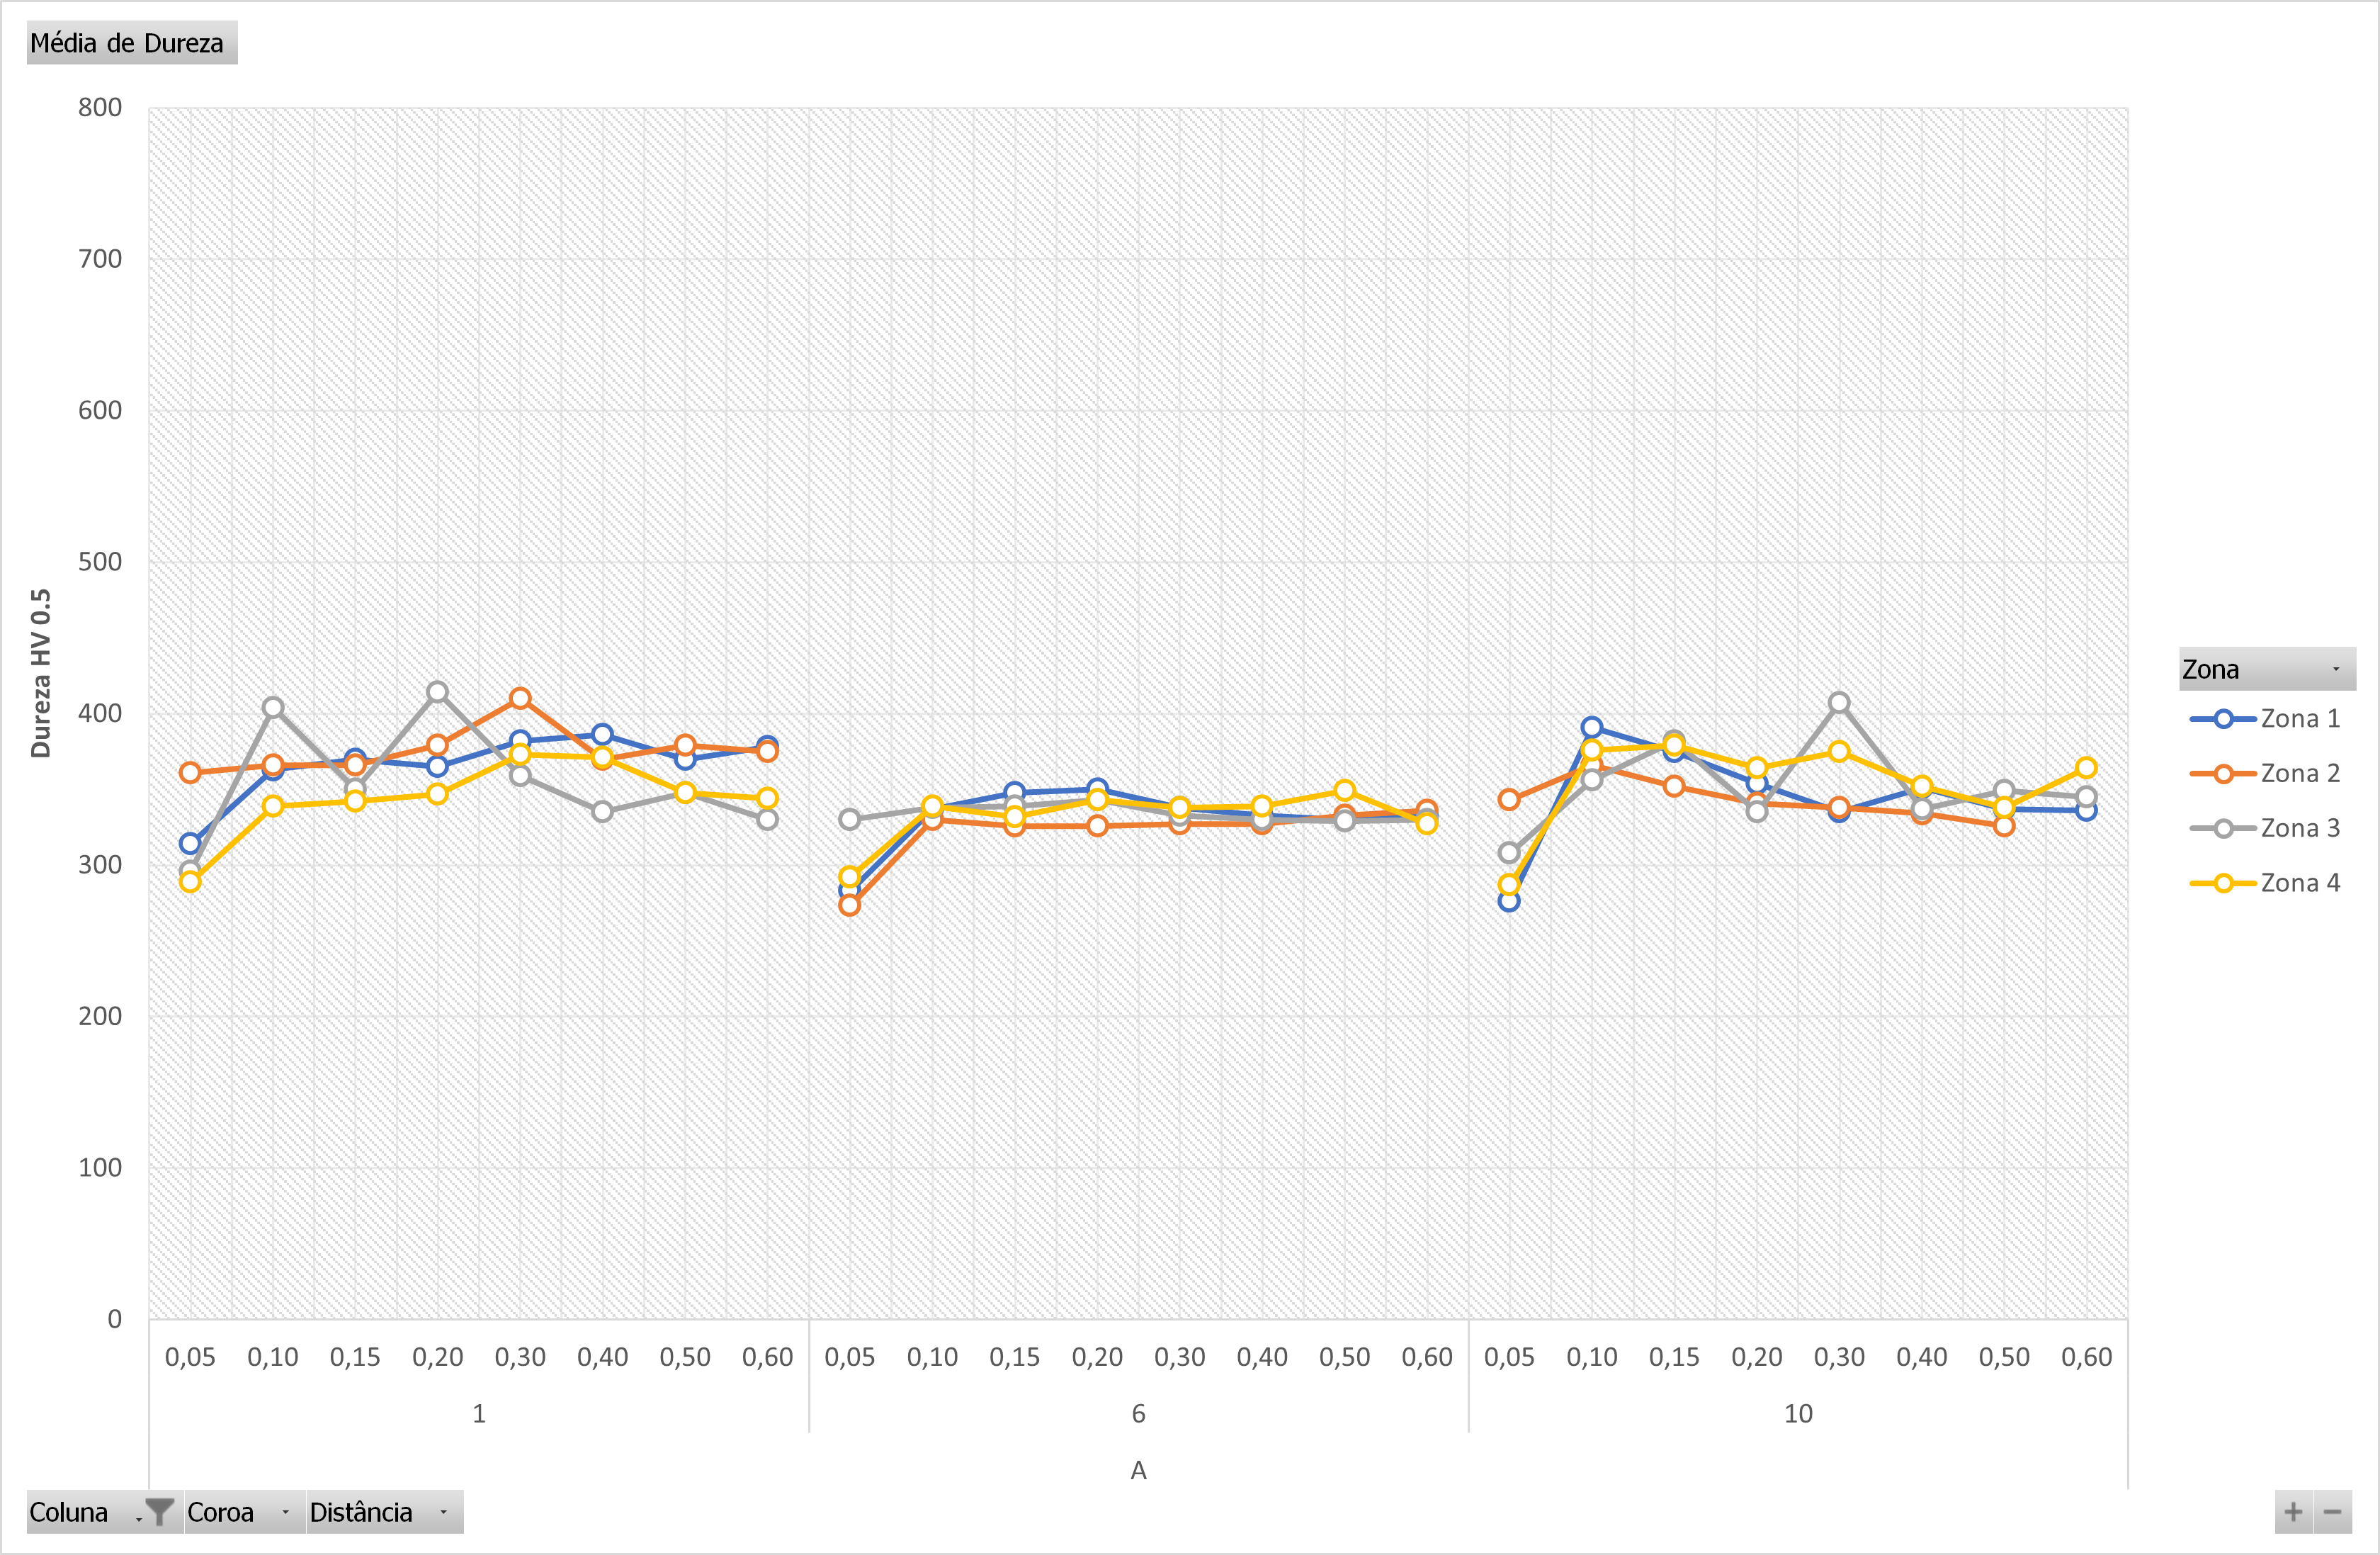
\includegraphics[width = 0.9\textwidth]{Figures/Cap4/Grafico_4_Zonas_Y.png}
        \caption{}
        \label{fig:resultados_Tampa_Y}
    \end{subfigure}%
    \begin{subfigure}{.4\textwidth}
        \centering
        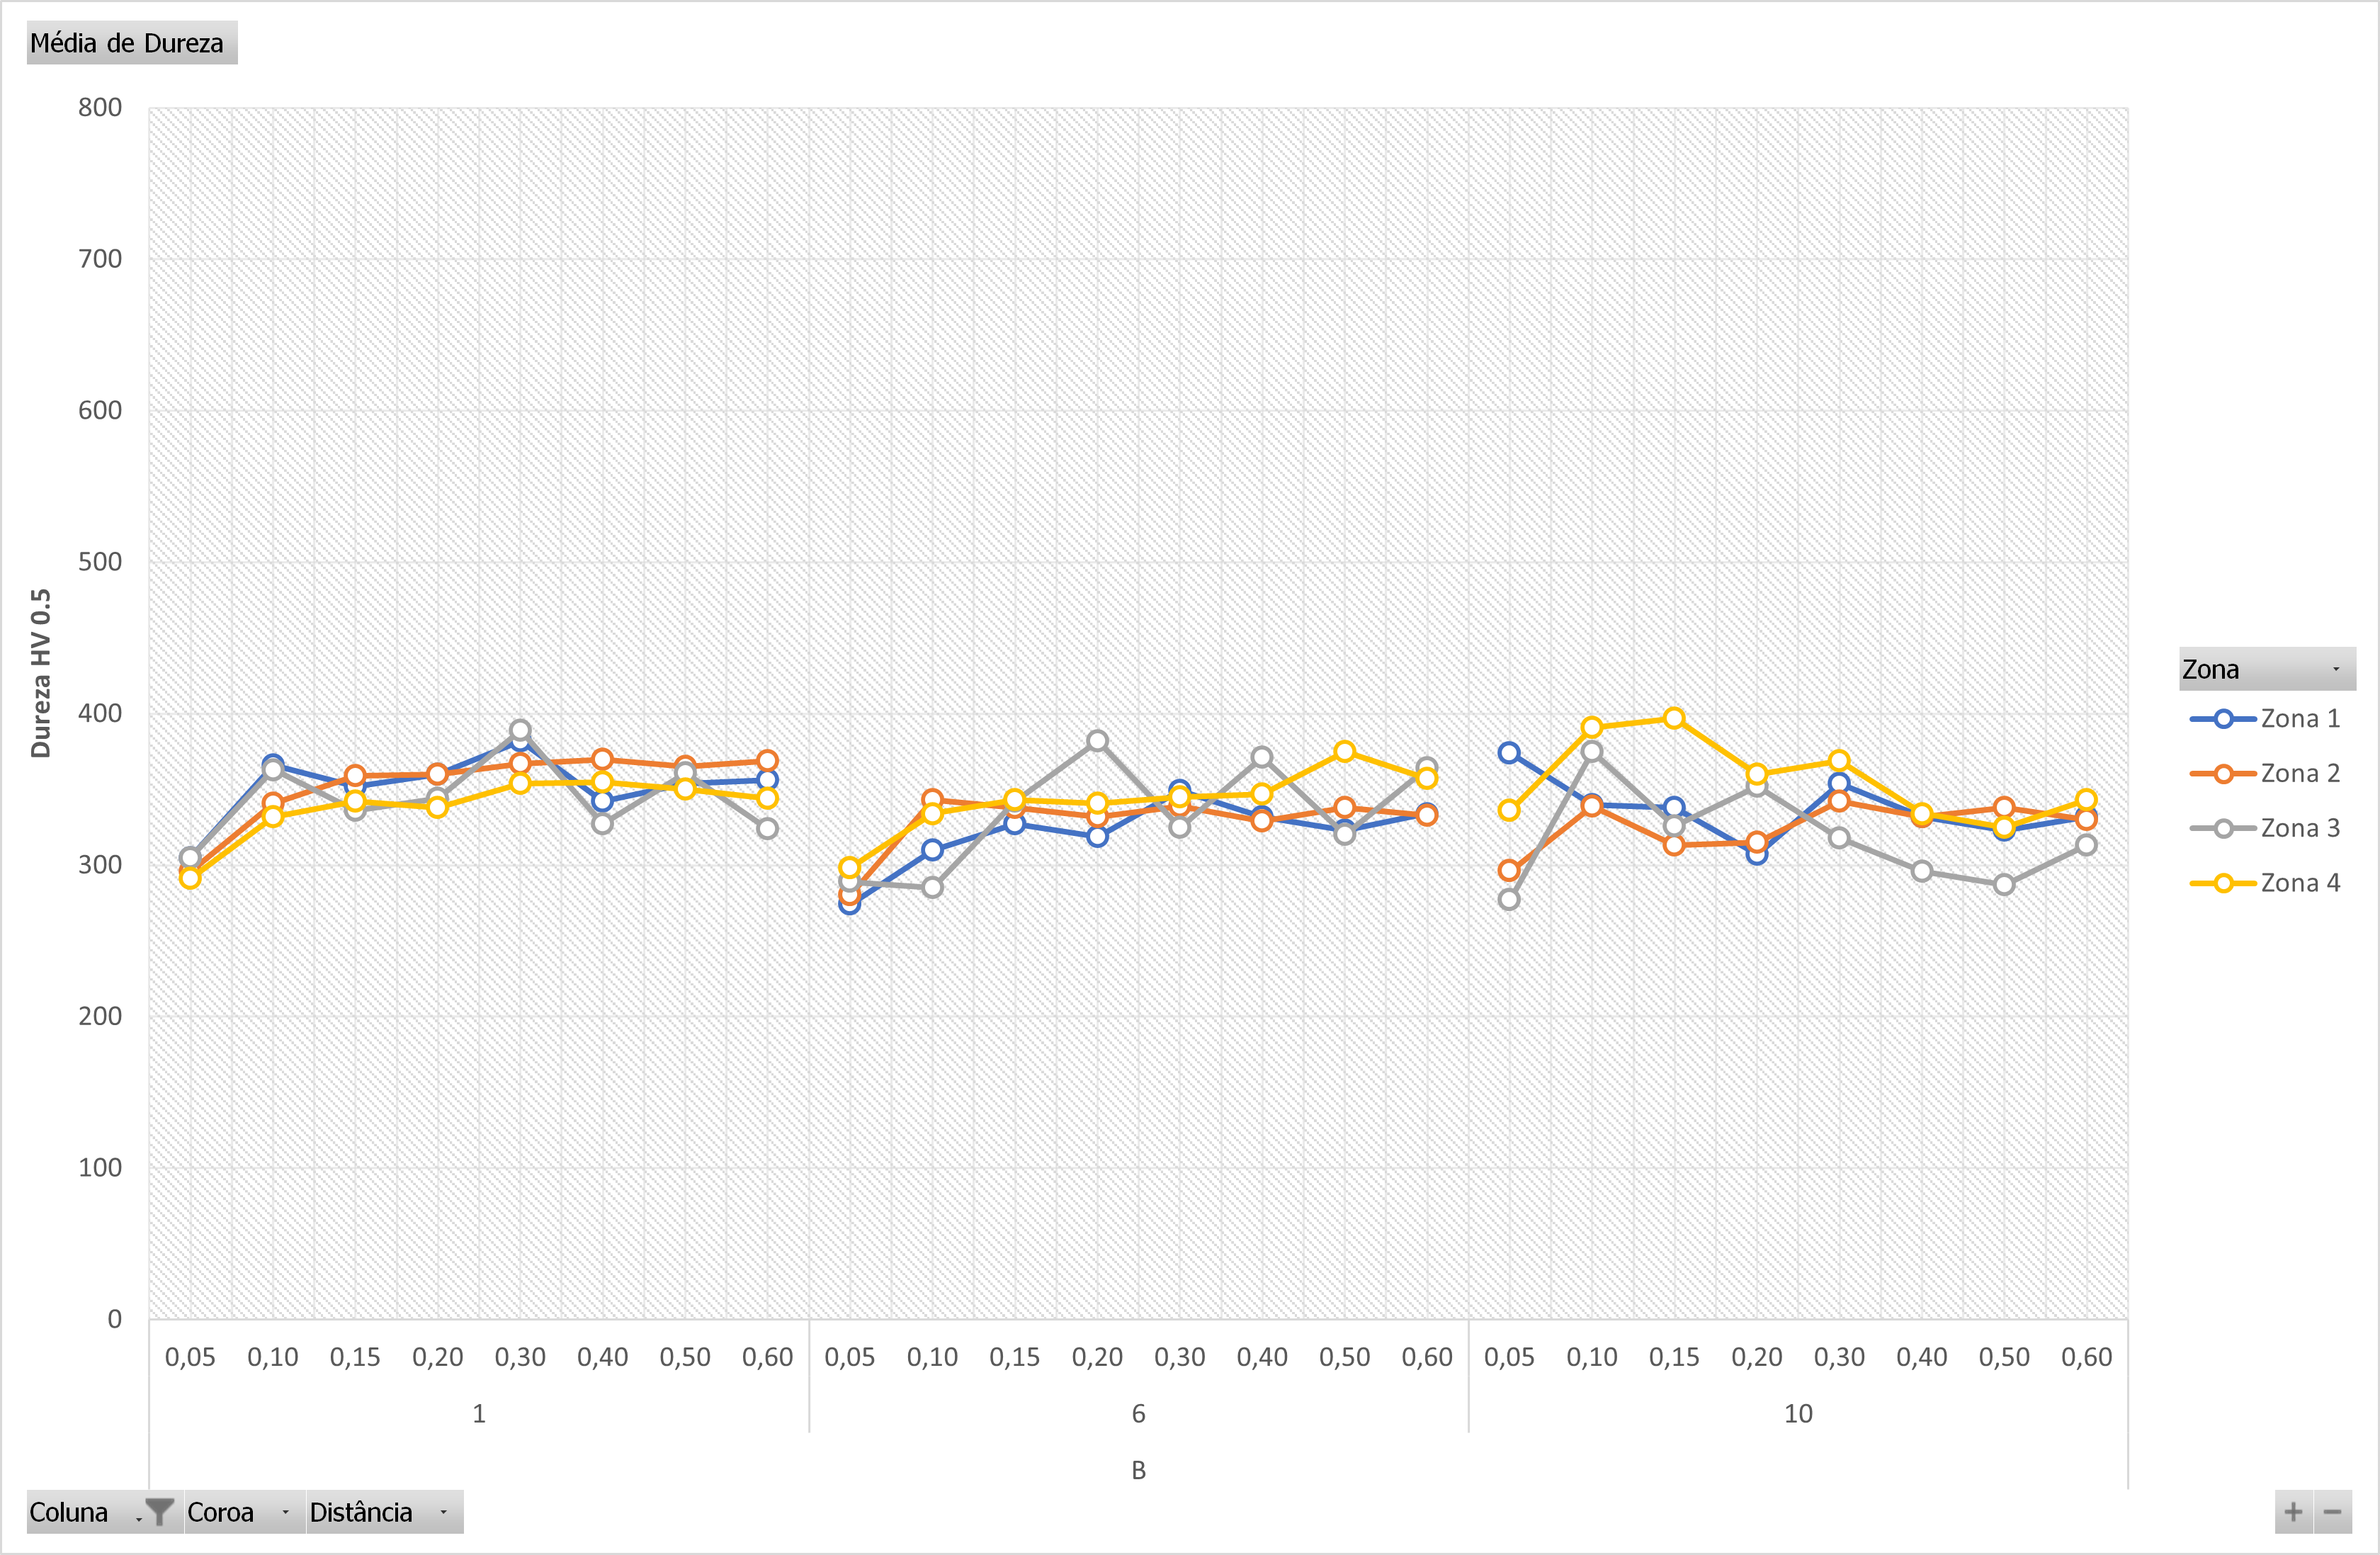
\includegraphics[width = 0.9\textwidth]{Figures/Cap4/Grafico_4_Zonas_O.png}
        \caption{}
        \label{fig:resultados_Tampa_O}
    \end{subfigure}
    \begin{subfigure}{.4\textwidth}\
        \centering
        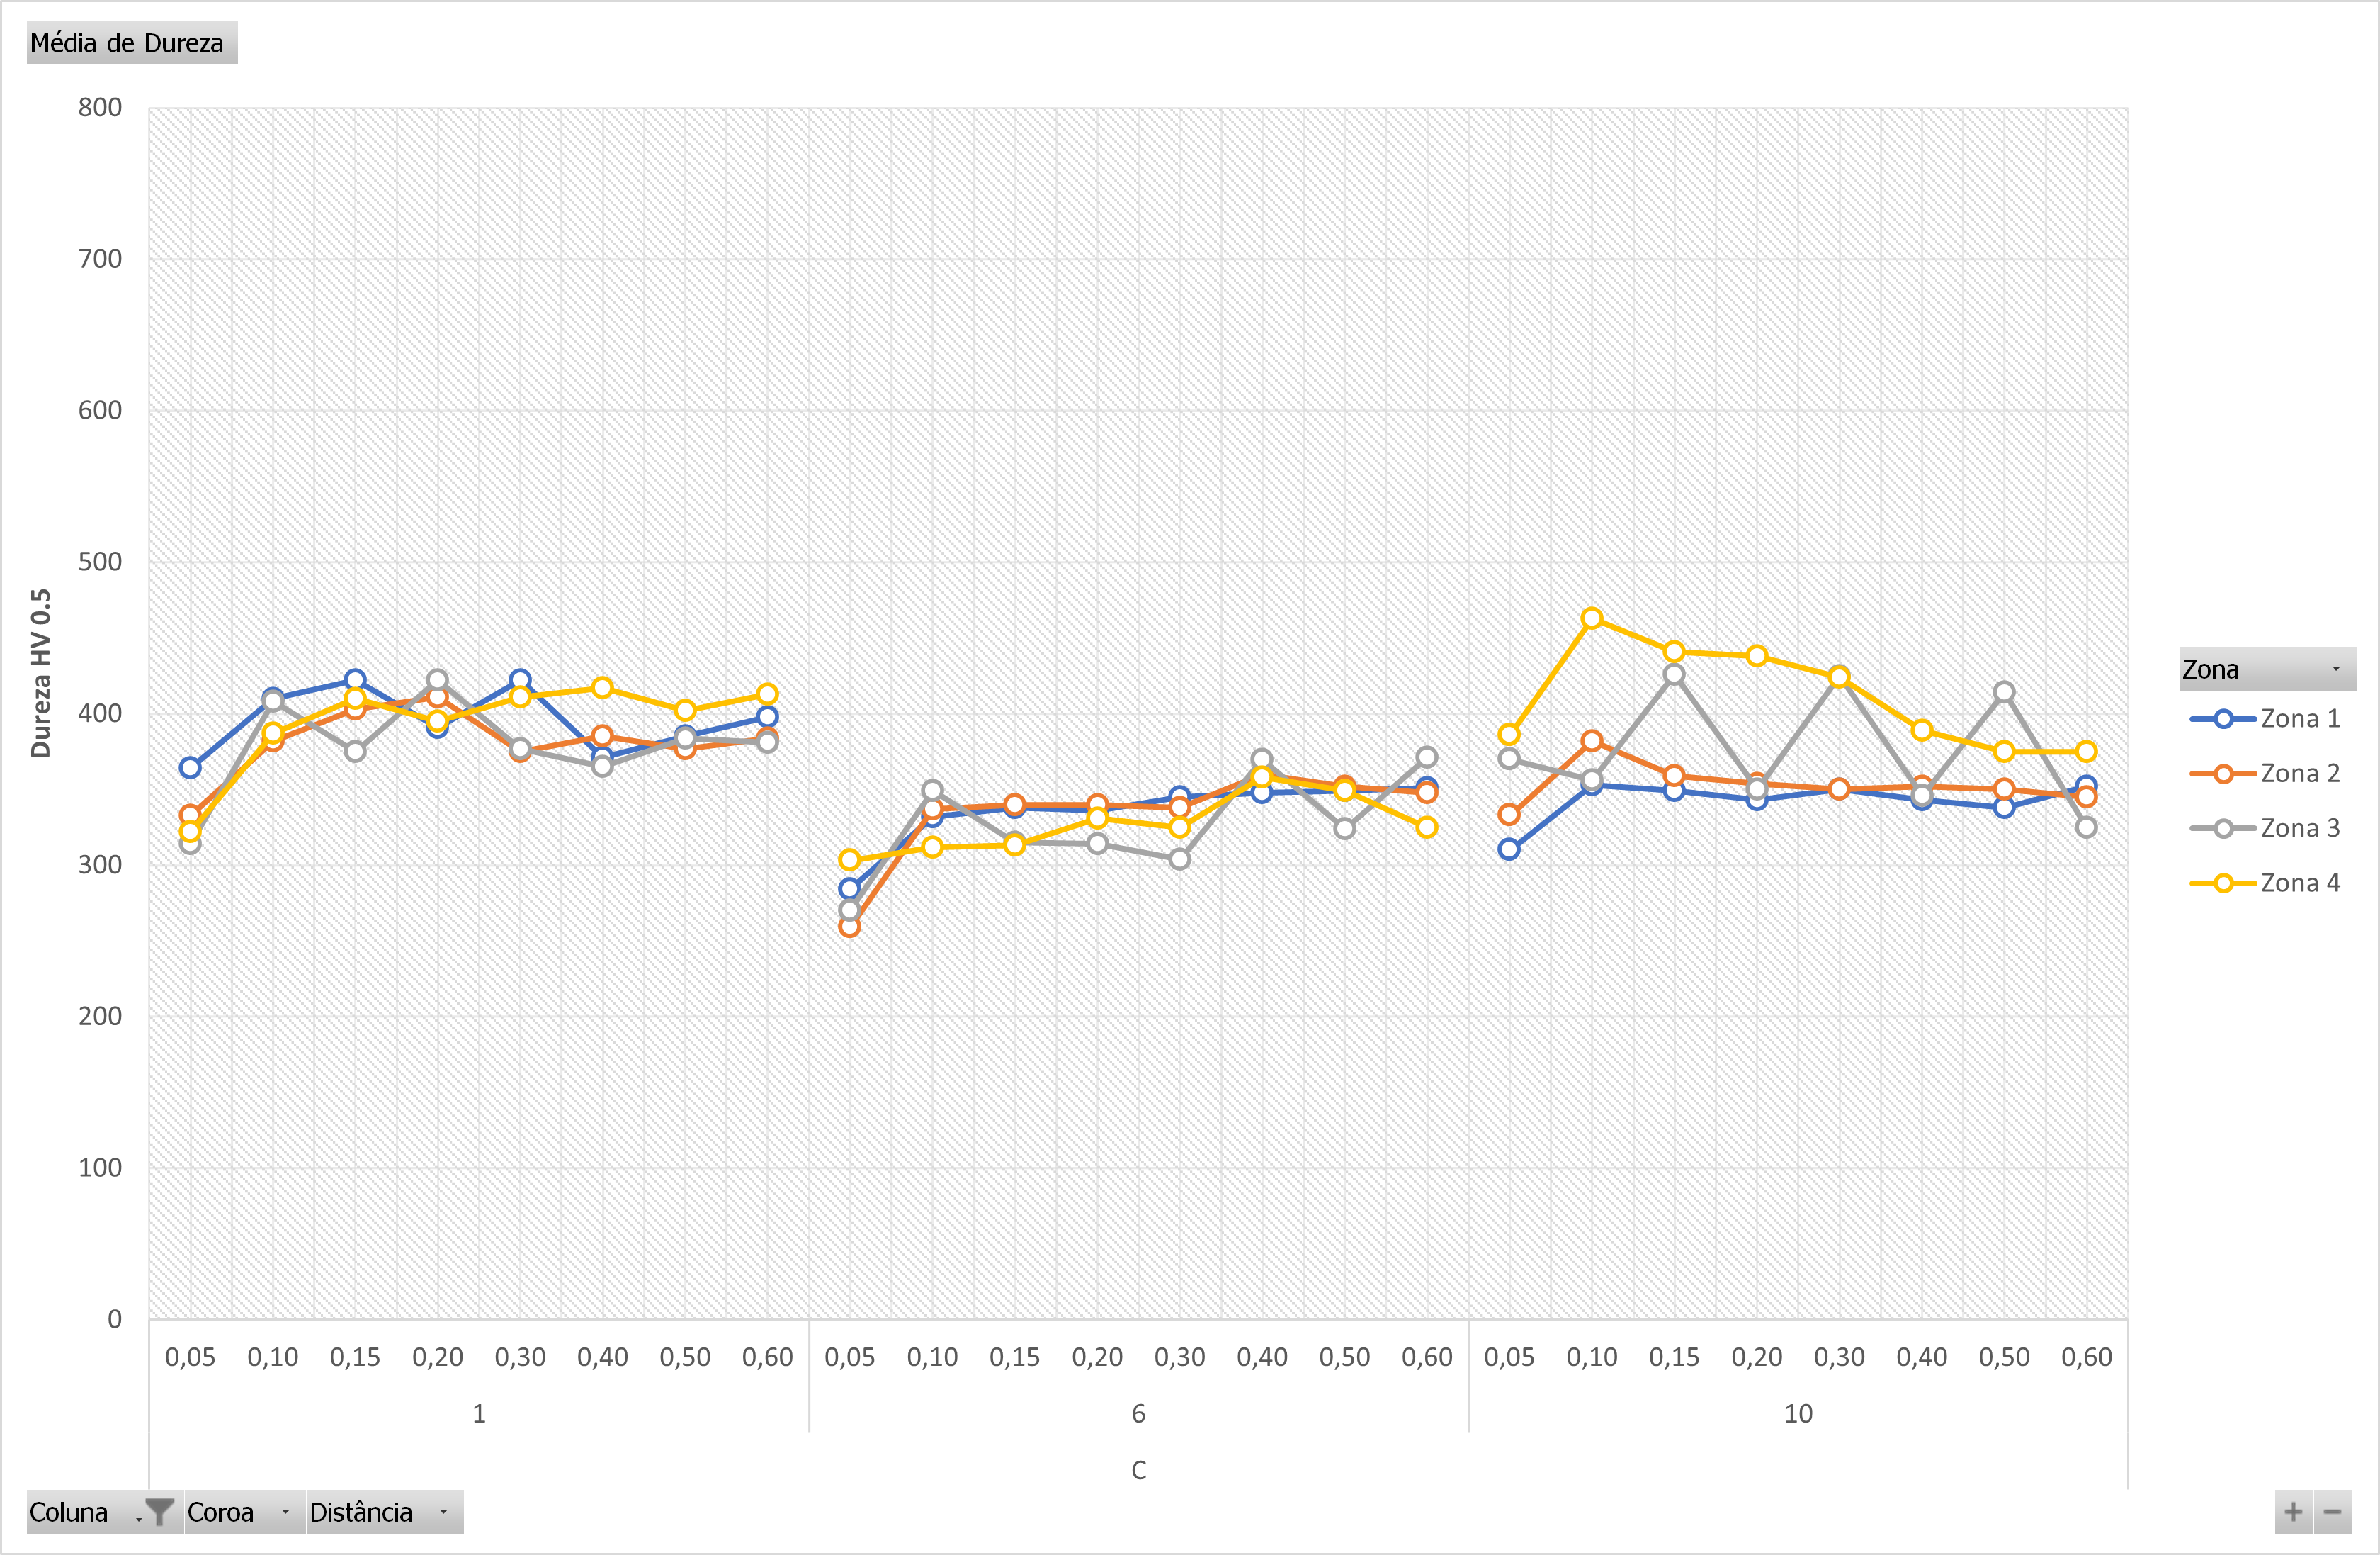
\includegraphics[width = 0.9\textwidth]{Figures/Cap4/Grafico_4_Zonas_P.png}
        \caption{}
        \label{fig:resultados_Tampa_P}
    \end{subfigure}%
    \begin{subfigure}{.4\textwidth}
        \centering
        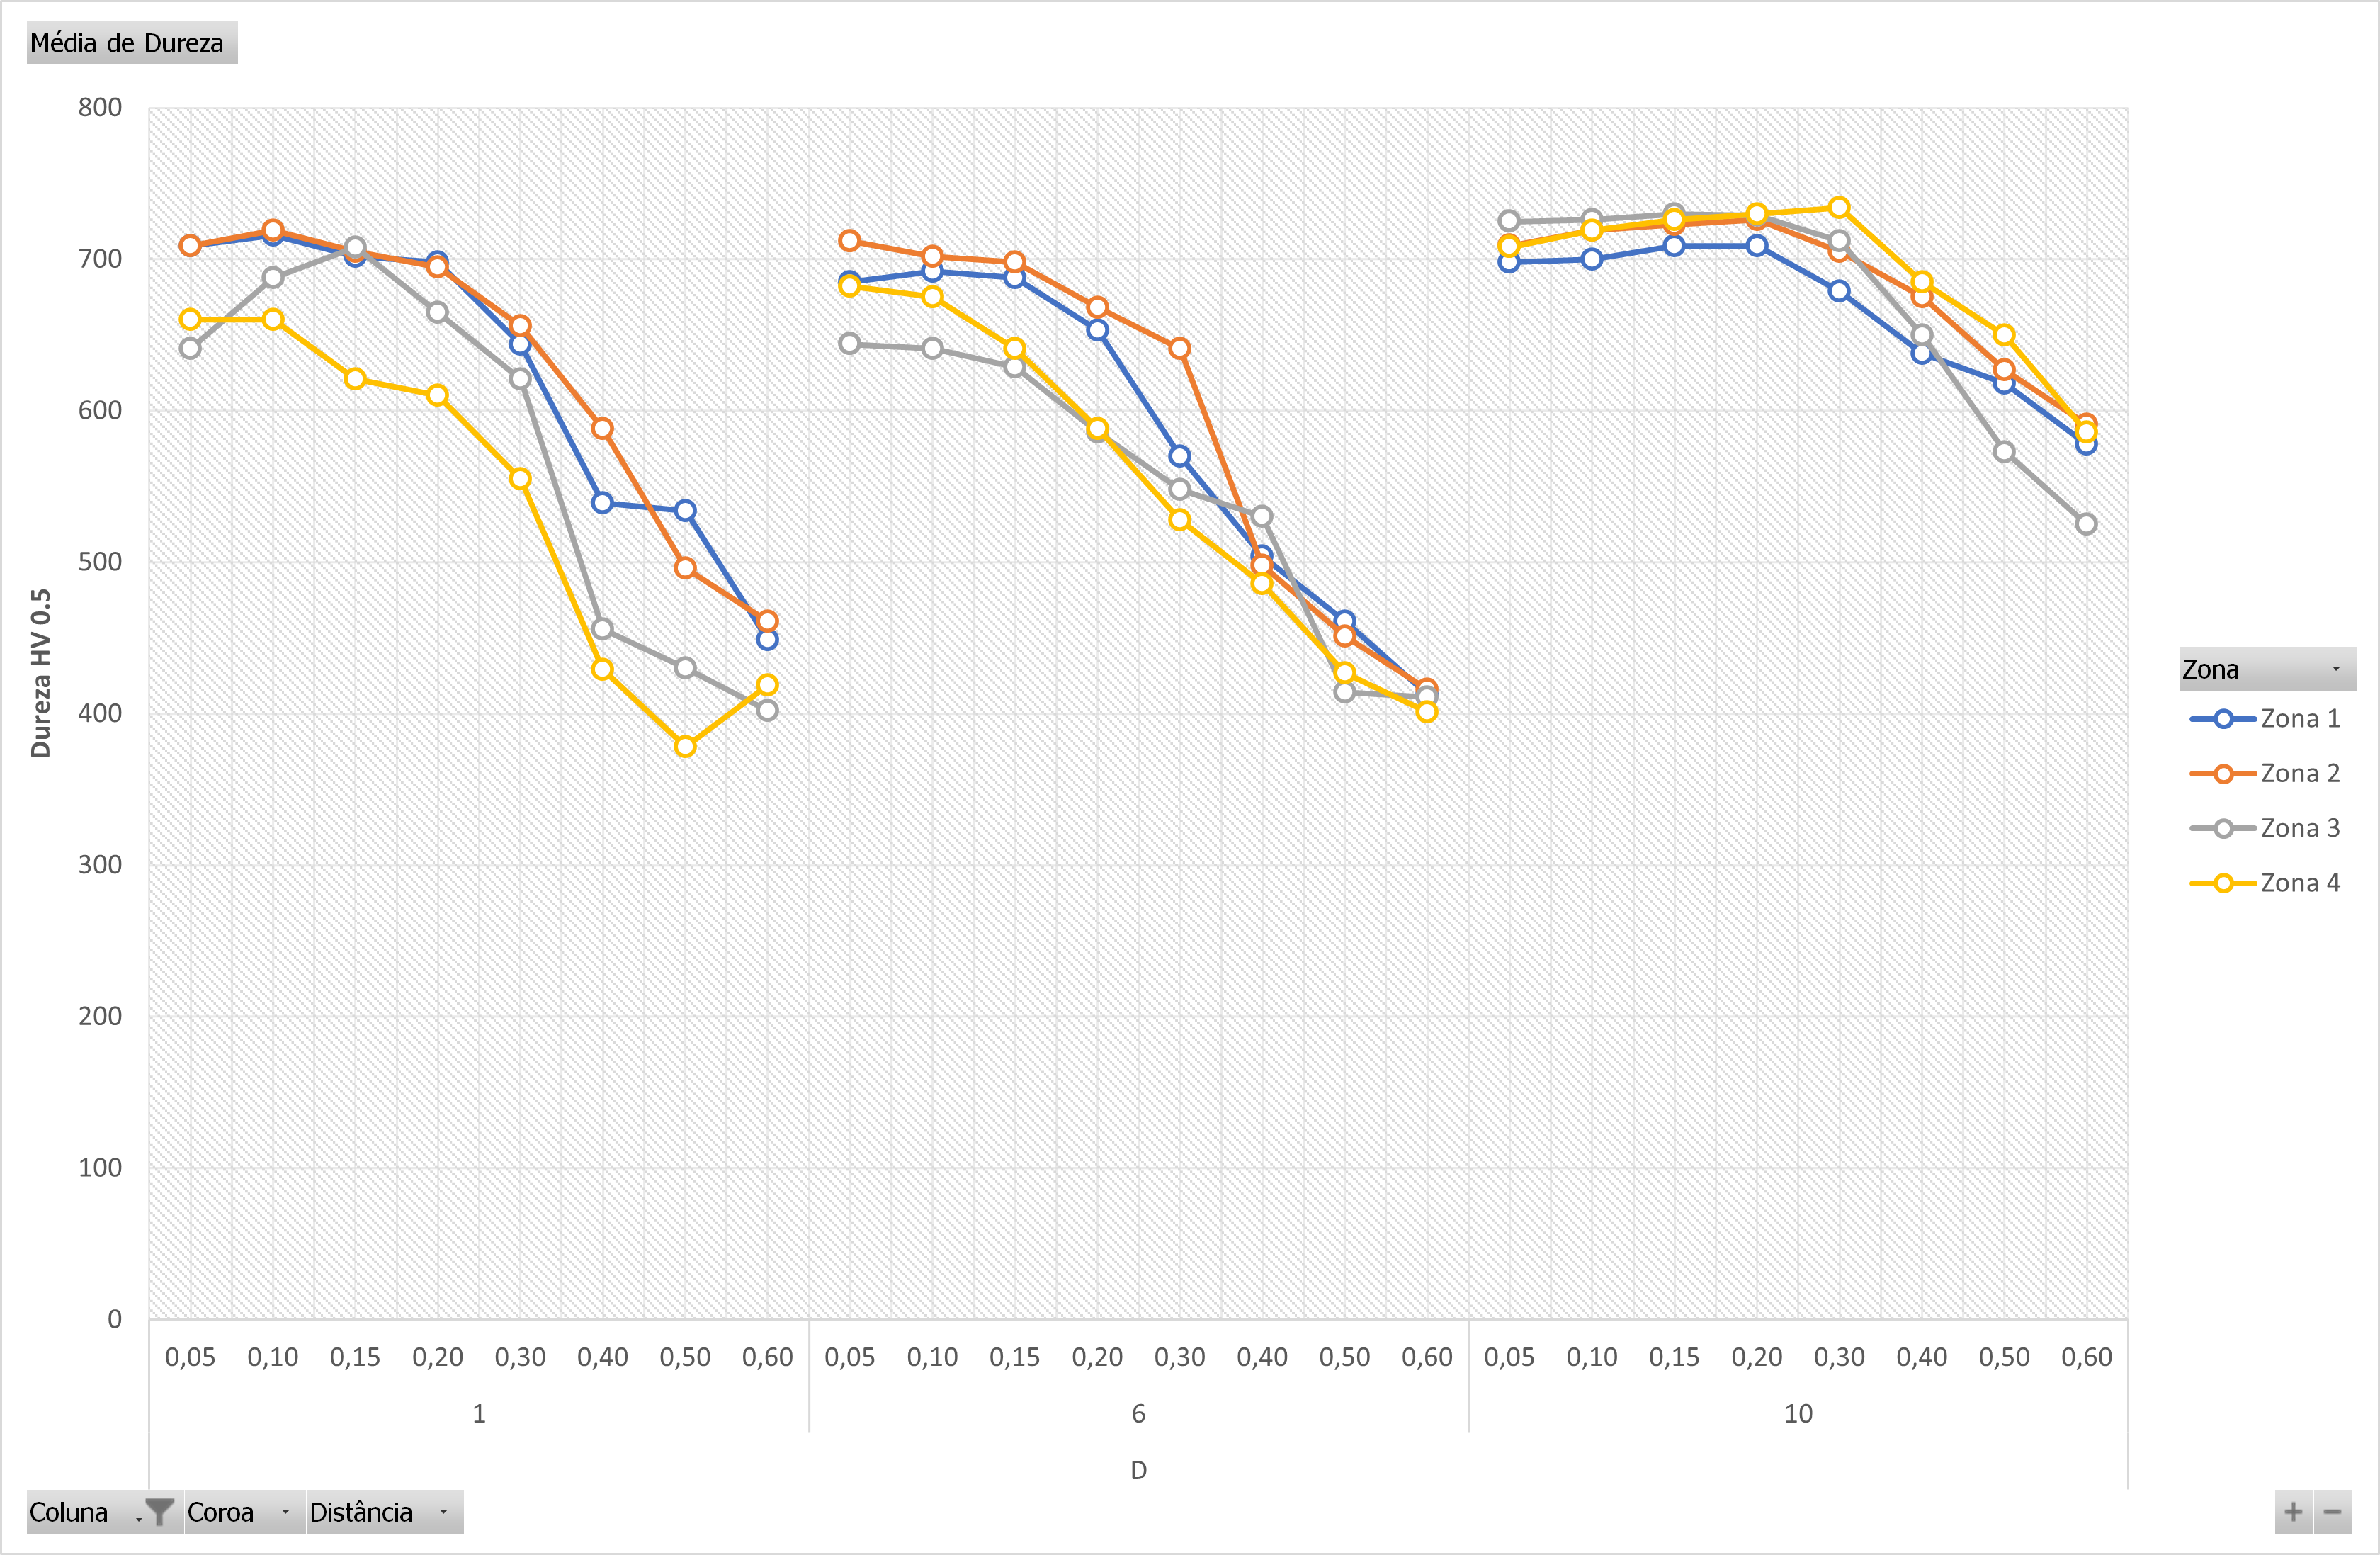
\includegraphics[width = 0.9\textwidth]{Figures/Cap4/Grafico_4_Zonas_ST.png}
        \caption{}
        \label{fig:resultados_ST}
    \end{subfigure}
    \caption[Filiações de dureza das quatro zonas na roda de coroa DB45 Nº 1]%
    {Gráficos das filiações de dureza das quatro zonas nas rodas de coroa protegidas por tampa Y, protegidas por tampa O, e protegida por tampa P, e sem tampa de proteção, respetivamente.}
\end{figure}
%%%%%%%%%%%%%%%%%%%%%%%%%%%%%%%%%%%%%%%%%%%%%%%%%%%%%%%%%%%%%%%%%%%%%%%%%%%%%
\newpage
\par
Observa-se claramente uma redução nos níveis de dureza em todos os tipos de ferramentas de proteção com tampa. No entanto, na ferramenta sem tampa, que protege apenas a parte inferior, não se observa uma alteração significativa nos níveis de dureza. Isso confirma duas teorias. Primeiro, que o uso de uma tampa é essencial para o funcionamento do sistema. E segundo, que a geometria da tampa não tem impacto significativo no resultado da proteção. É importante mencionar que não foi proposta uma solução que dispensasse a proteção na parte inferior, uma vez que o fluido de têmpera é carregado de baixo para cima no tanque de têmpera, o que poderia resultar na remoção da tampa pelo fluido de têmpera e possíveis danos ao sistema de têmpera. Novamente, nas Figuras \ref{fig:resultados_4T_dent}, não são observadas alterações significativas nas durezas do dentado em nenhuma das soluções propostas.
%%%%%%%%%%%%%%%%%%%%%%%%%%%%%%%%%%%%%%%%%%%%%%%%%%%%%%%%%%%%%%%%%%%%%%%%%%%%%
\begin{figure}[htb]
    \centering
    \begin{subfigure}{.4\textwidth}\
        \centering
        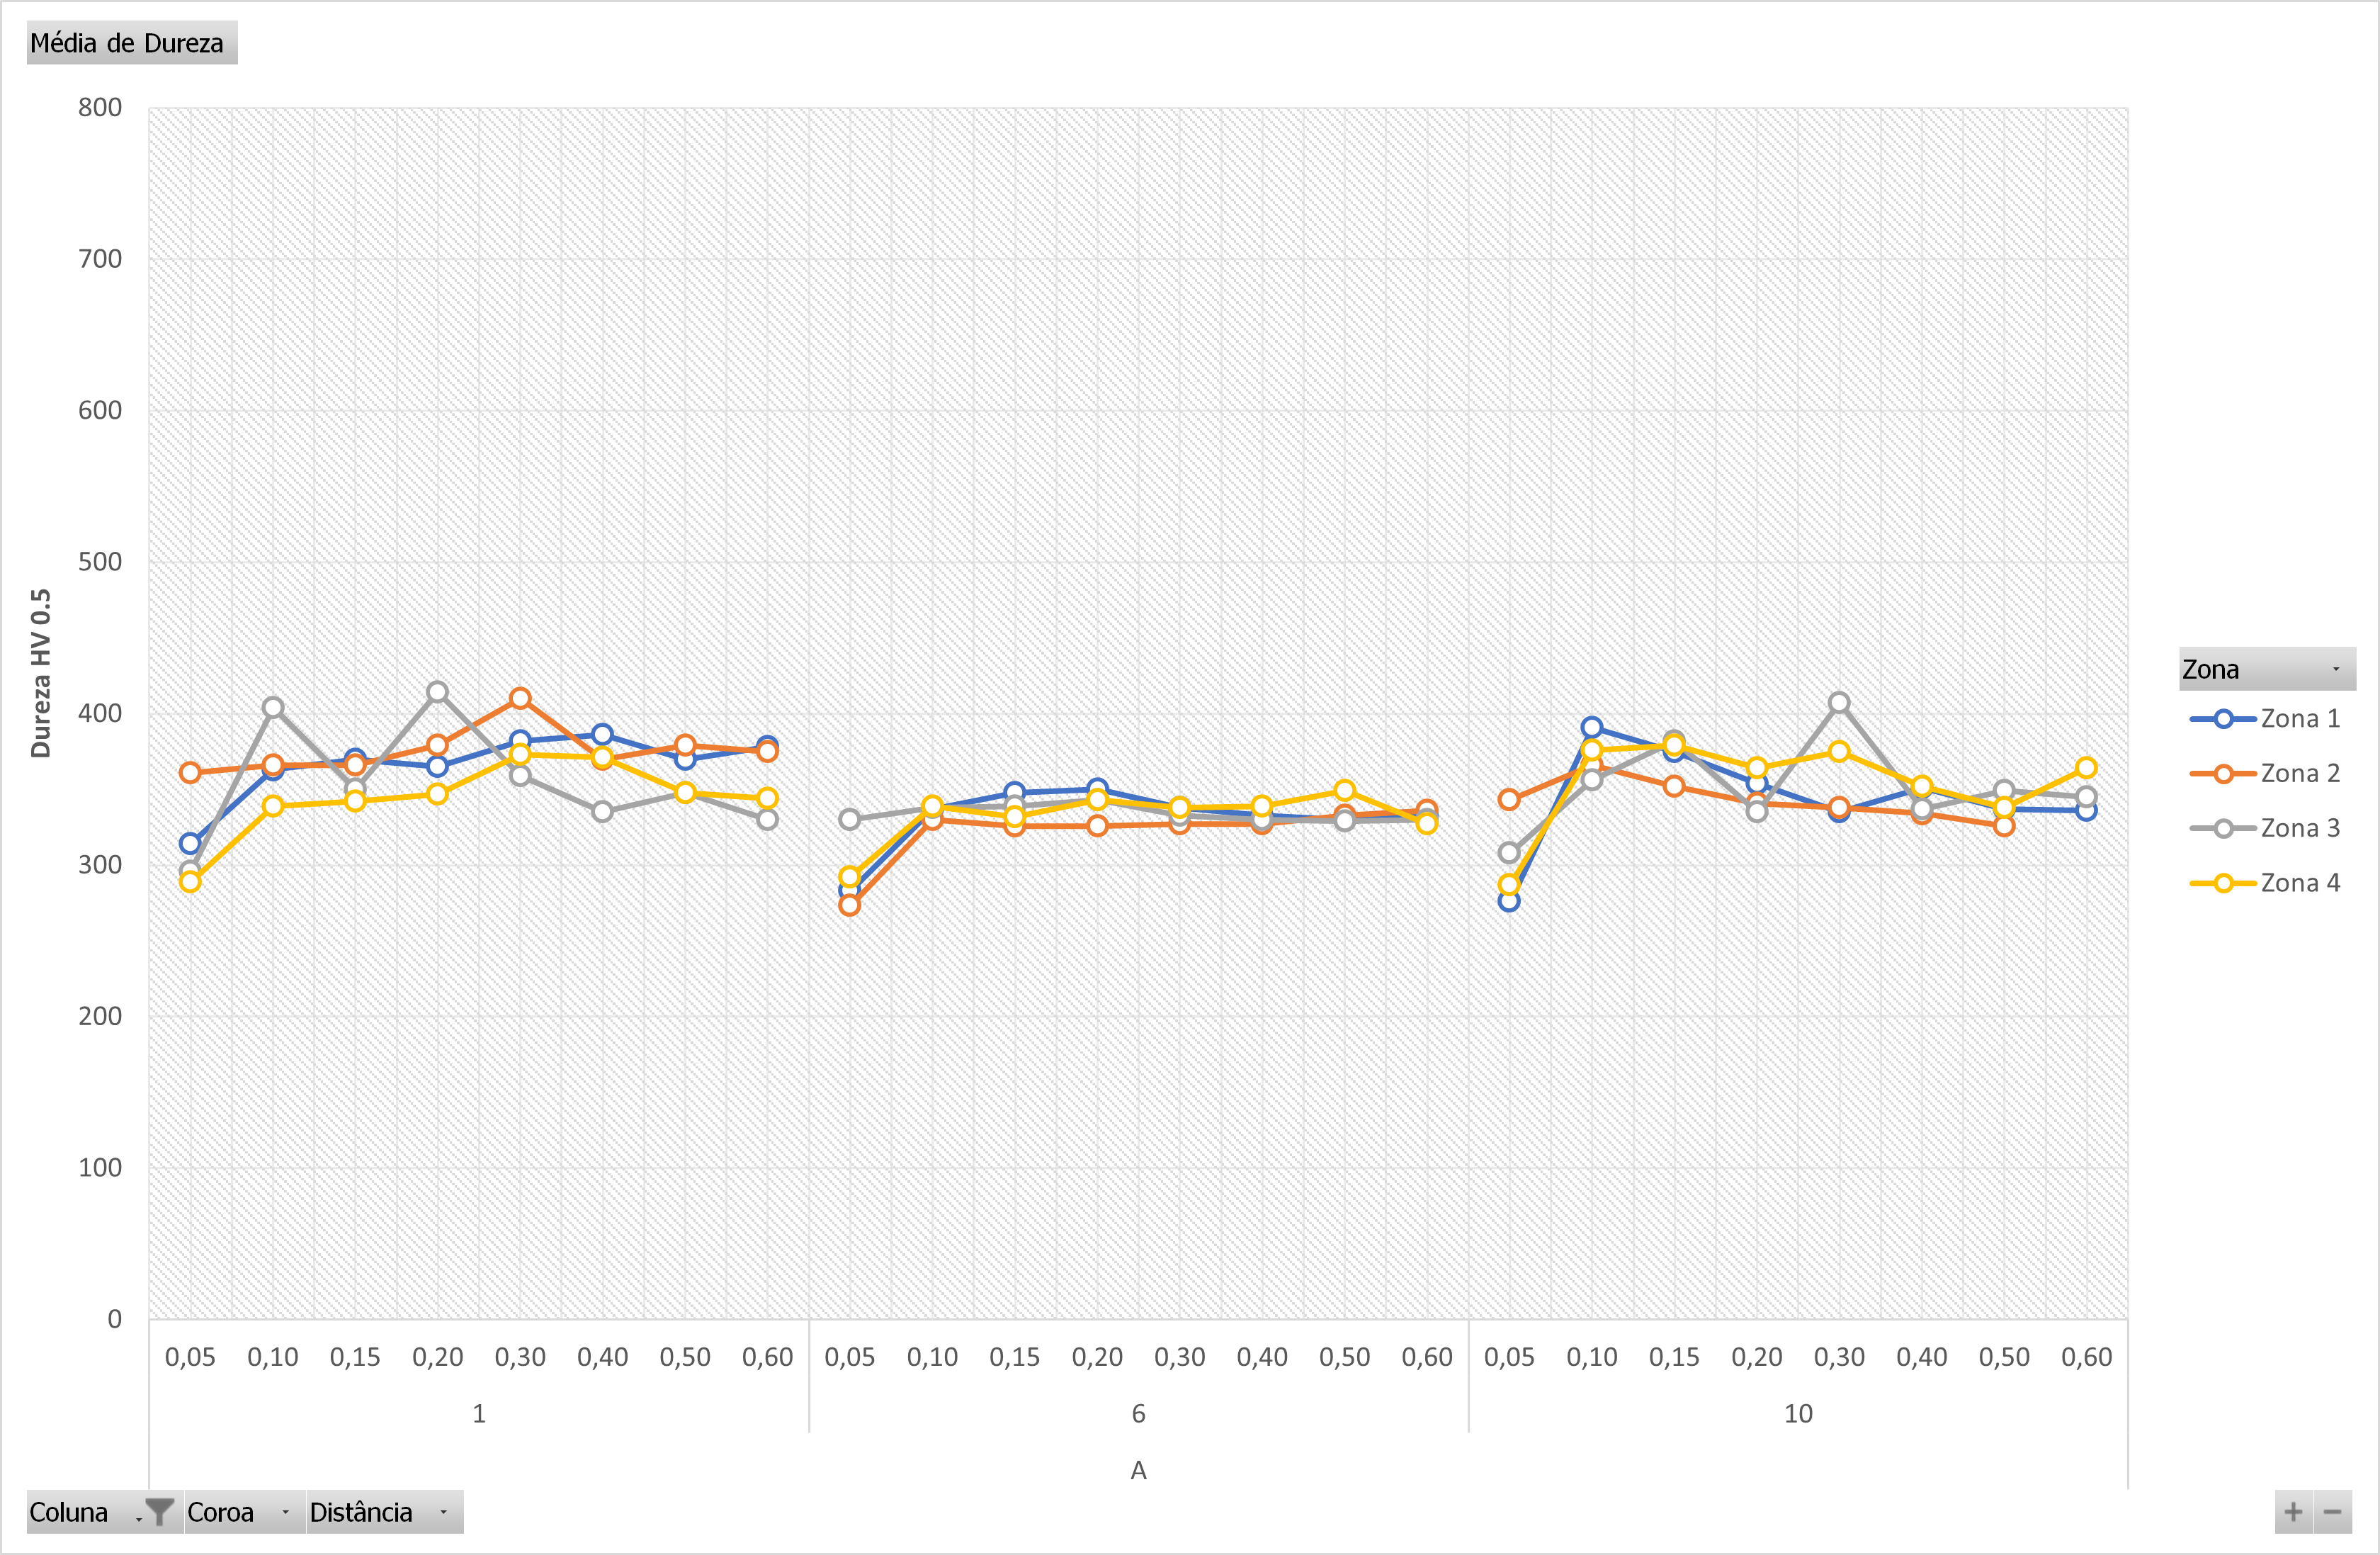
\includegraphics[width = 0.9\textwidth]{Figures/Cap4/Grafico_4_Zonas_Y.png}
        \caption{}
        \label{fig:resultados_Tampa_Y_dent}
    \end{subfigure}%
    \begin{subfigure}{.4\textwidth}
        \centering
        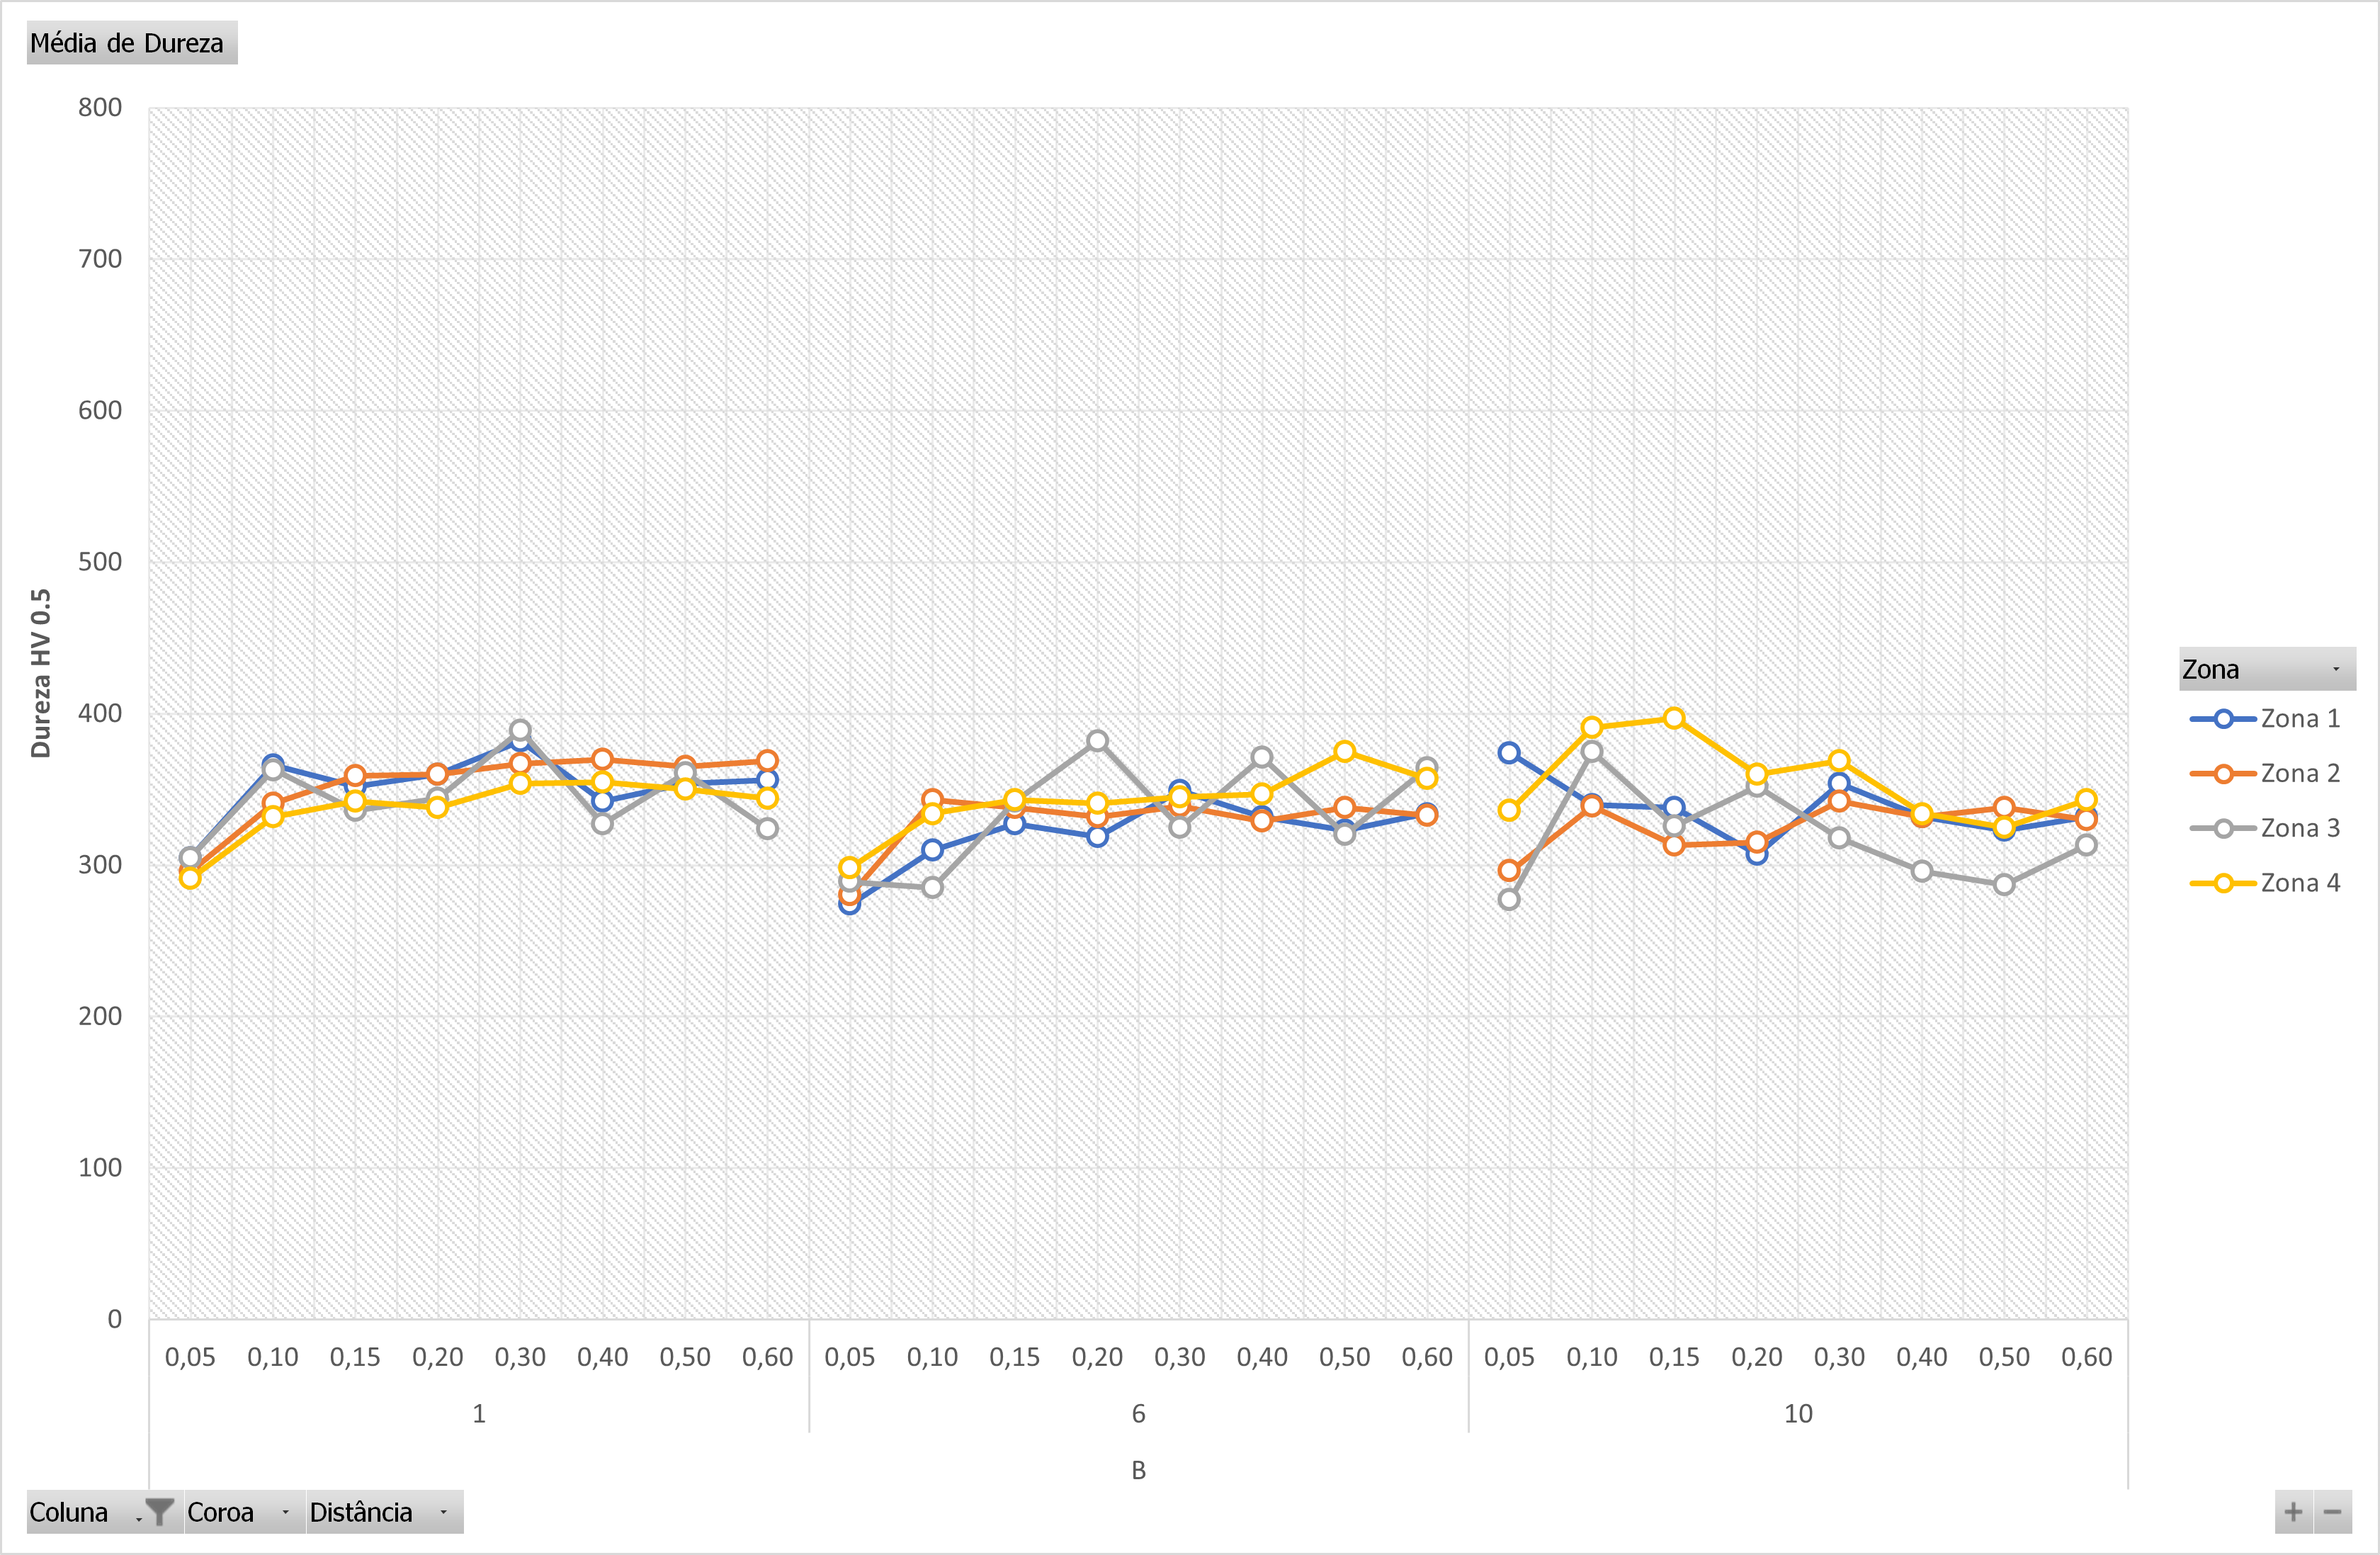
\includegraphics[width = 0.9\textwidth]{Figures/Cap4/Grafico_4_Zonas_O.png}
        \caption{}
        \label{fig:resultados_Tampa_O_dent}
    \end{subfigure}
    \begin{subfigure}{.4\textwidth}\
        \centering
        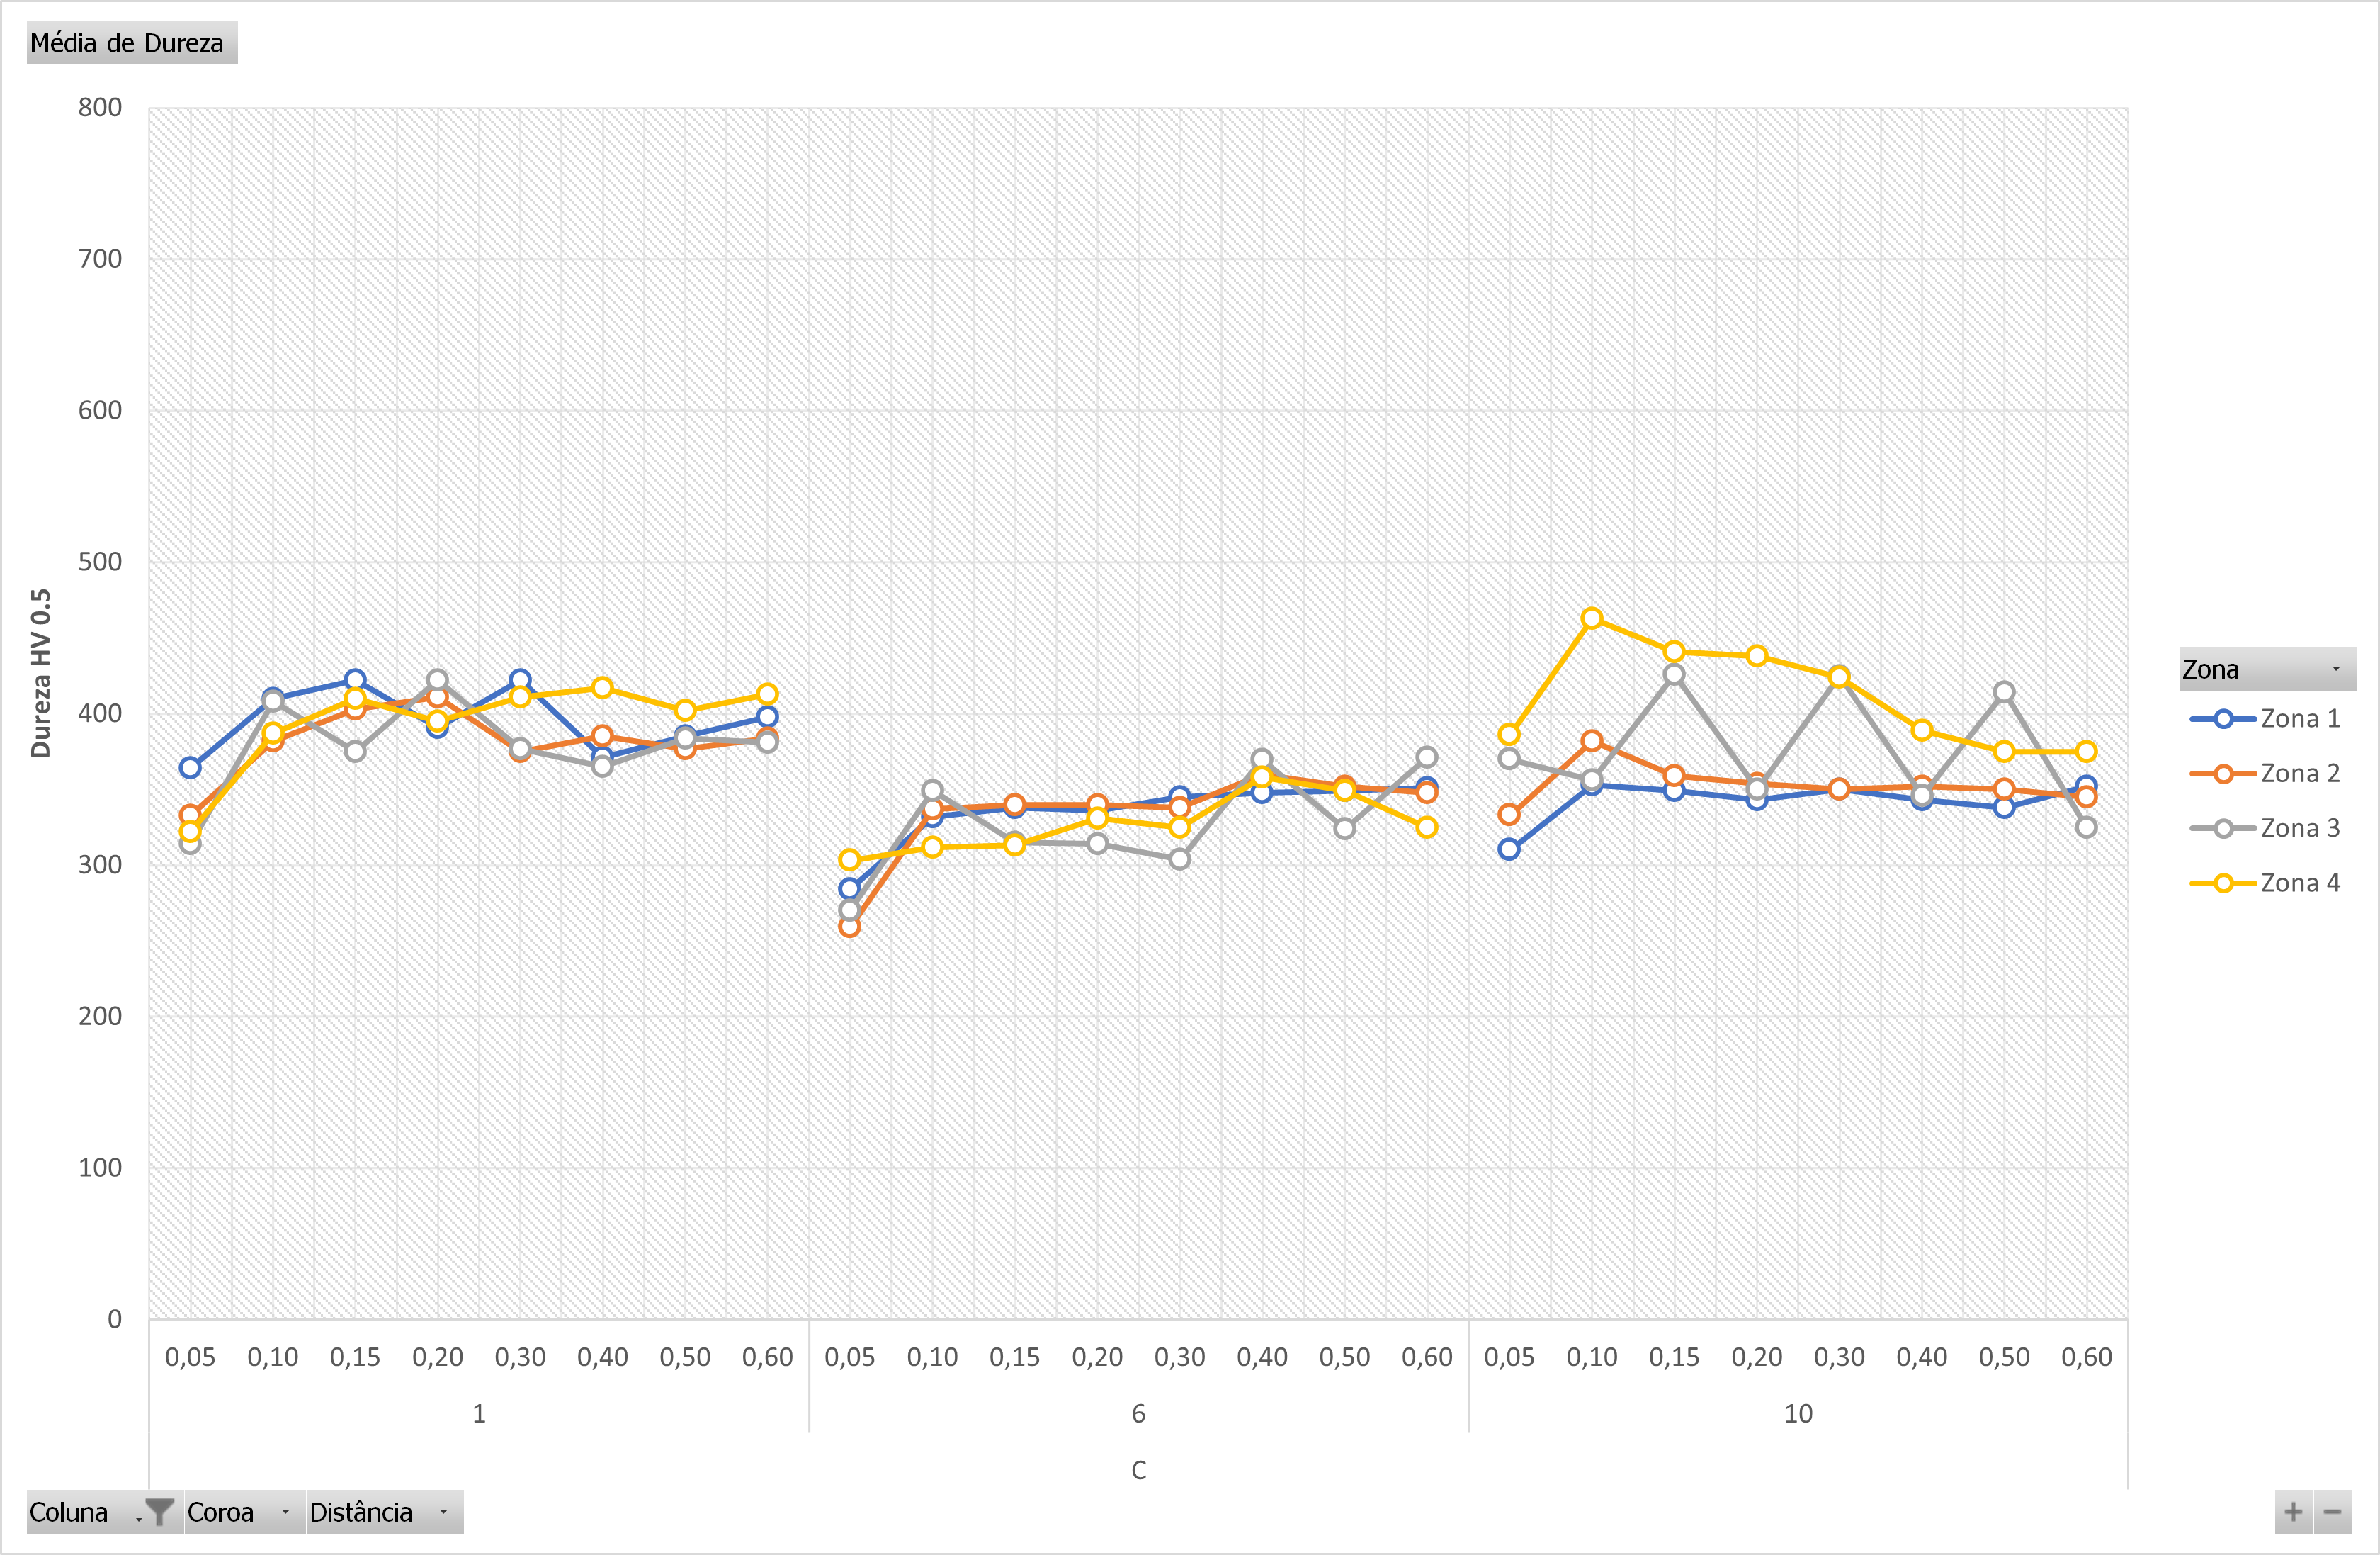
\includegraphics[width = 0.9\textwidth]{Figures/Cap4/Grafico_4_Zonas_P.png}
        \caption{}
        \label{fig:resultados_Tampa_P_dent}
    \end{subfigure}%
    \begin{subfigure}{.4\textwidth}
        \centering
        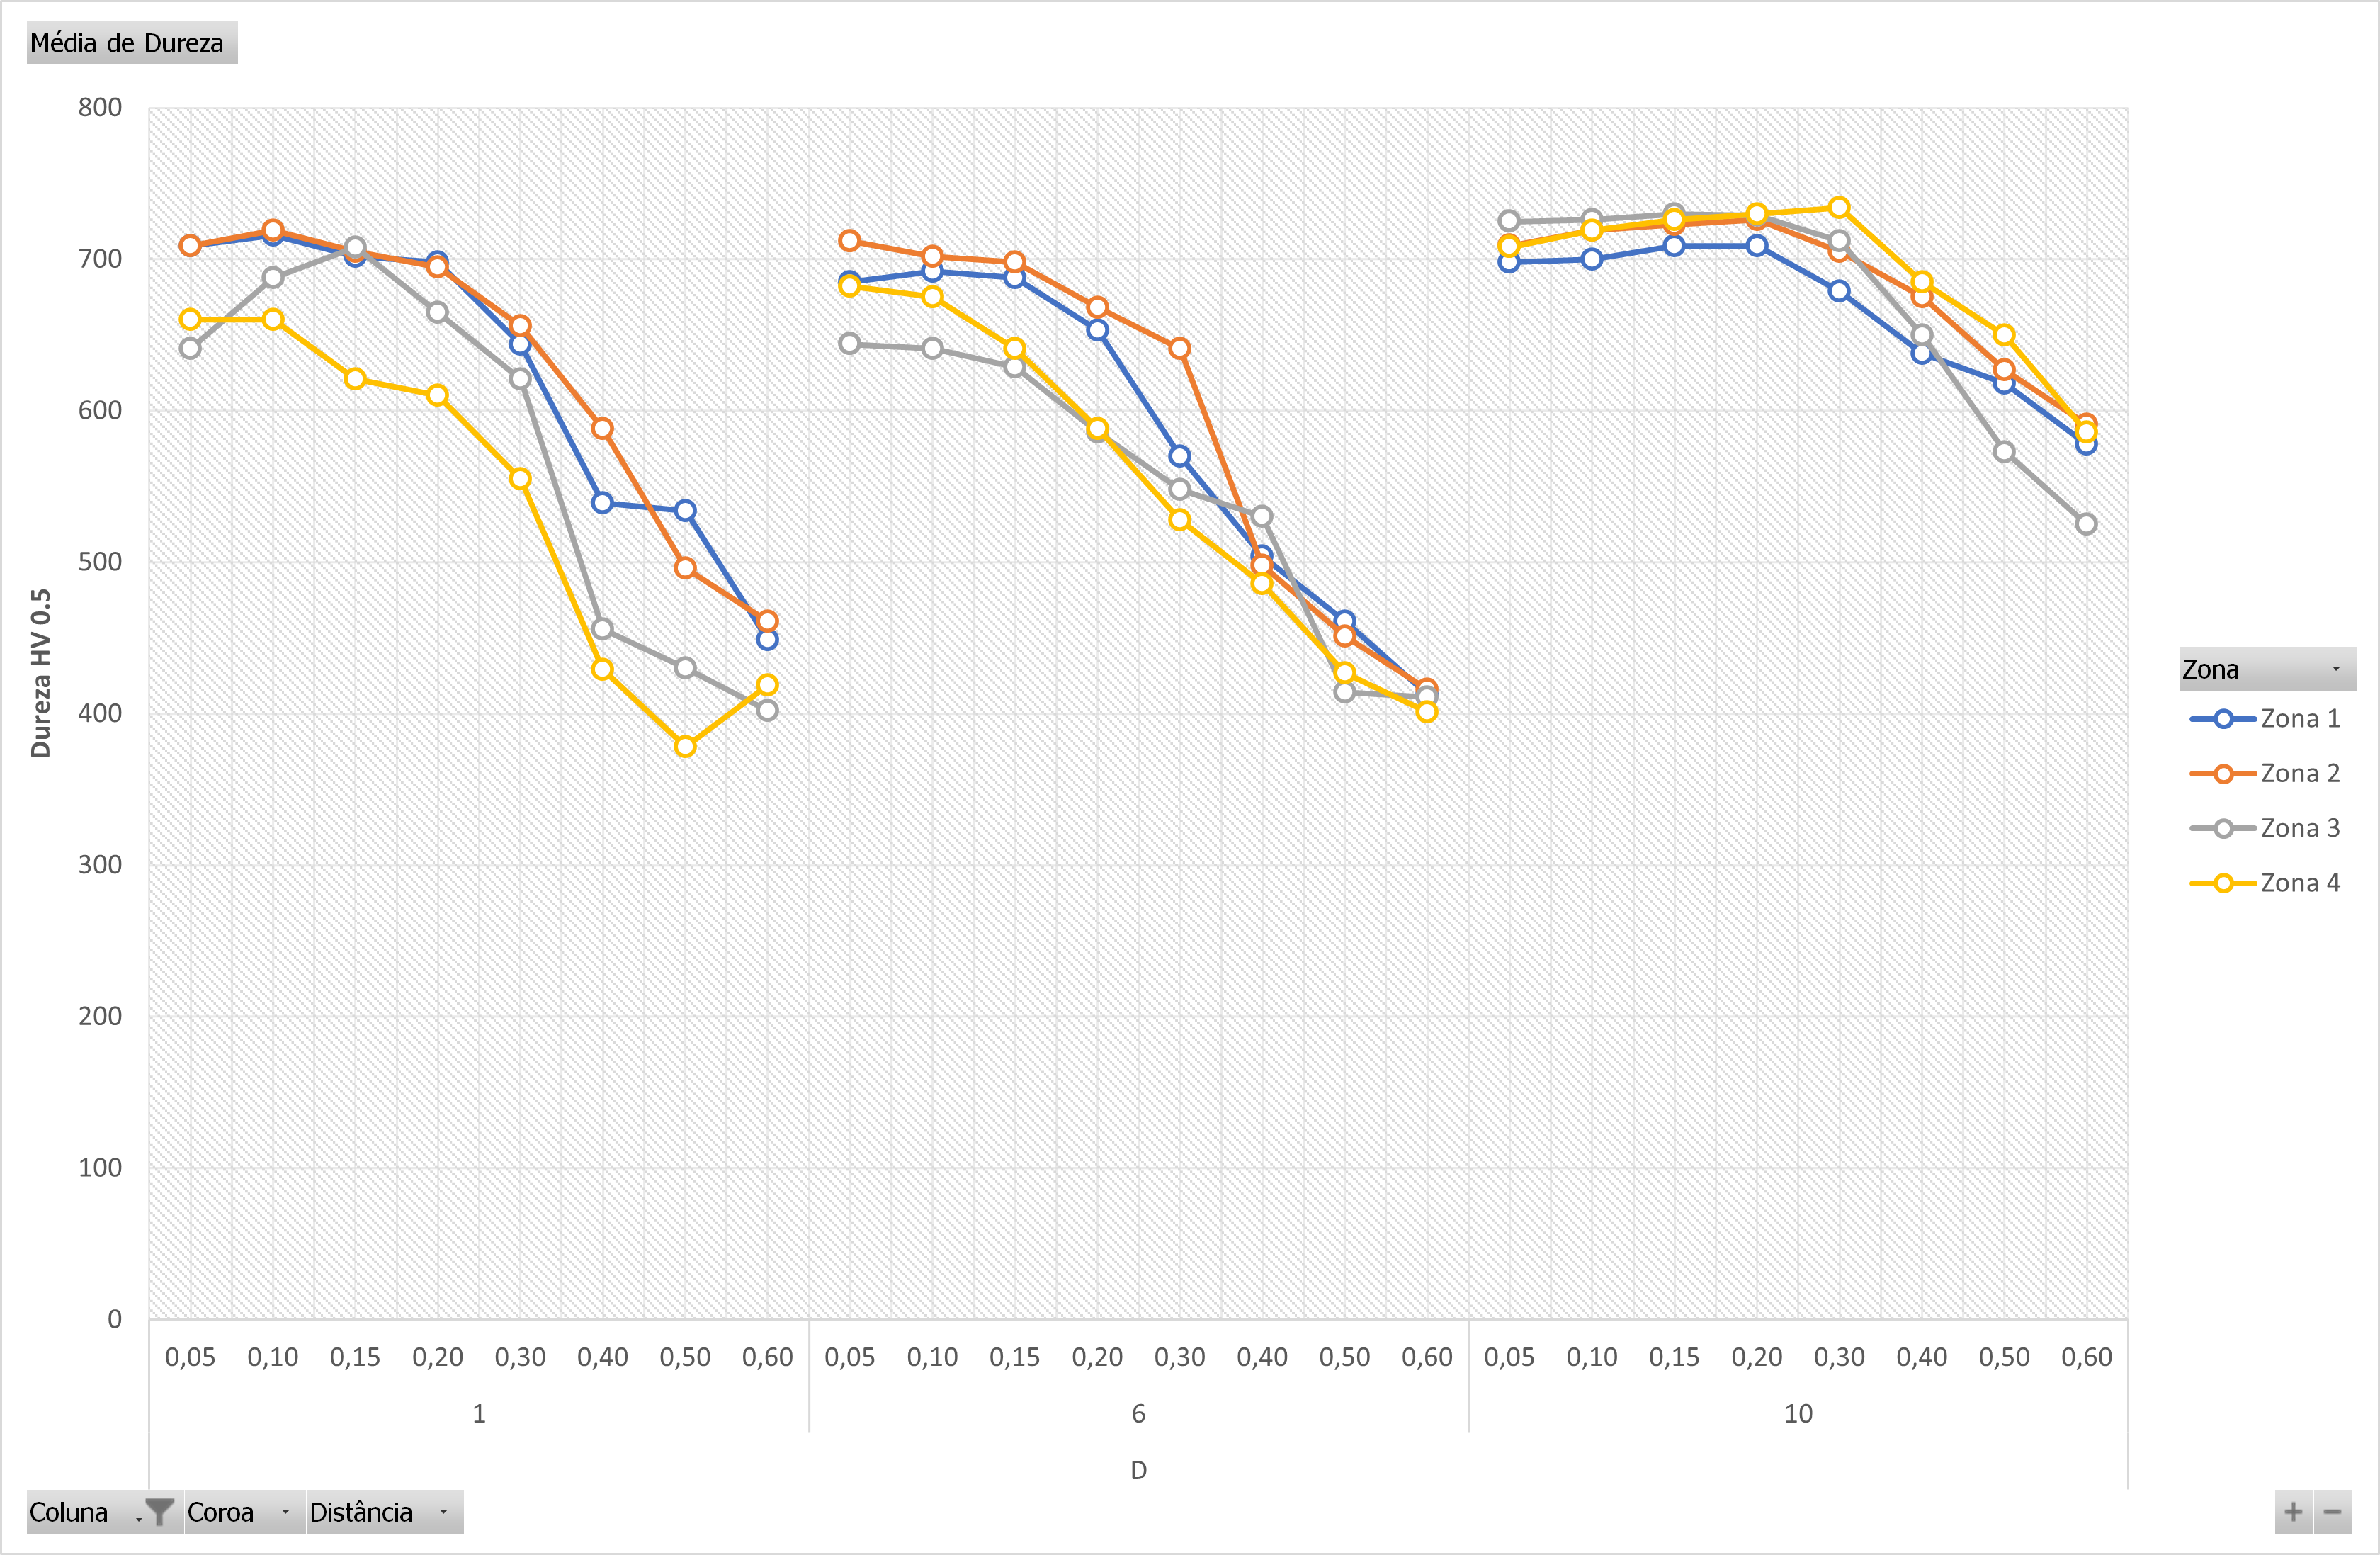
\includegraphics[width = 0.9\textwidth]{Figures/Cap4/Grafico_4_Zonas_ST.png}
        \caption{}
        \label{fig:resultados_ST_dent}
    \end{subfigure}
    \caption[Filiações de dureza das quatro zonas na roda de coroa DB45 Nº 1]%
    {Gráficos das filiações de dureza das quatro zonas nas rodas de coroa protegidas por tampa Y, protegidas por tampa O, e protegida por tampa P, e sem tampa de proteção, respetivamente.}
    \label{fig:resultados_4T_dent}
\end{figure}
%%%%%%%%%%%%%%%%%%%%%%%%%%%%%%%%%%%%%%%%%%%%%%%%%%%%%%%%%%%%%%%%%%%%%%%%%%%%%
\section{Resultados da Espectroscopia} \label{sec:resultados_espectroscopia}
